\documentclass[british,titlepage]{ntnuthesis}

\title{An NTNU Thesis \LaTeX{} Document Class}
\shorttitle{An NTNU Thesis Document Class}
\author{Community of Practice in Computer Science Education at NTNU}
\shortauthor{CoPCSE$@$NTNU}
\date{CC-BY \ntnuthesisdate}

\addbibresource{thesis.bib}


% From https://www.overleaf.com/learn/latex/Glossaries

\makeglossaries % Prepare for adding glossary entries


\newglossaryentry{latex}
{
        name=latex,
        description={Is a mark up language specially suited for
scientific documents}
}

\newglossaryentry{bibliography}
{
        name=bibliography,
        plural=bibliographies,
        description={A list of the books referred to in a scholarly work,
typically printed as an appendix}
}

\newglossaryentry{maths}
{
    name=mathematics,
    description={Mathematics is what mathematicians do}
}

\newglossaryentry{desksim}
{
    name=DeskSim,
    description={The current simulator used by Lokførerskolen today}
}

\newglossaryentry{lokforerskolen}
{
    name=Lokførerskolen,
    description={The Norwegian Train Driver Academy, a vocational school educating train drivers, and the client of this project}
}

\newglossaryentry{scrum}
{
    name=Scrum,
    description={An agile framework for project management within software development}
}

\newglossaryentry{kanban}
{
    name=Kanban,
    description={A framework for agile software development which focuses on balancing demands with available capacity}
}

\newglossaryentry{sprint}
{
    name=sprint,
    description={A short period where a team aims to complete a set amount of work withing the Scrum methodology}
}

\newglossaryentry{jira}
{
    name=Jira,
    description={A web service for tracking and managing product development, developed by Atlassian}
}

\newglossaryentry{jmonkeyengine}
{
    name=jMonkeyEngine,
    description={A 3D game engine written in Java by jME Core Team in 2003}
}

\newglossaryentry{unity}
{
    name=Unity,
    description={A cross-platform game engine developed by Unity Technologies}
}

\newglossaryentry{unrealengine}
{
    name=Unreal Engine,
    description={A 3D game and computer graphics engine developed by Epic Games}
}

\newglossaryentry{godot}
{
    name=Godot,
    description={An open source, cross-platform game engine}
}

\newglossaryentry{cryengine}
{
    name=CryEngine,
    description={A 3D game engine developed by Crytek}
}

\newglossaryentry{open3dengine}
{
    name=Open 3D Engine,
    description={An open source 3D game engine managed by The Linux Foundation}
}

\newglossaryentry{opensource}
{
    name=open source,
    description={Computer software released publicly and freely for anyone to modify, use and/or publish}
}

\newglossaryentry{crossplatform}
{
    name=cross platform,
    description={The practice of developing the same software for multiple technologies or environments}
}

\newglossaryentry{github}
{
    name=GitHub,
    description={A service for hosting software repositories and version control using Git}
}

\newglossaryentry{garbagecollection}
{
    name=garbage collection,
    description={When the compiler frees up memory by deleting unused or obsolete  memory references}
}

\newglossaryentry{gizmo}
{
    name=gizmo,
    description={An overlay with a functional purpose, providing visually relevant options to the user}
}

\newglossaryentry{mesh}
{
    name=mesh,
    description={A graphic primitive, represented as geometric shapes when rendered}
}

\newglossaryentry{viewport}
{
    name=viewport,
    description={The area on the screen visible to the user}
}

\newglossaryentry{blueprint}
{
    name=blueprint,
    description={Unreal Engine's own node-based programming language for visual scripting}
}

\newglossaryentry{heads-updisplay}
{
    name=heads-up display,
    description={Elements overlaying the screen, displaying information to the user}
}

\newglossaryentry{spline}
{
    name=spline,
    description={A mathematical function for interpolating smoothly between multiple points, creating a customizable curve}
}

\newglossaryentry{actor}
{
    name=actor,
    description={A base class for any object that can be placed into a level in Unreal Engine}
}

\newglossaryentry{instanced dynamic material}
{
    name=instanced dynamic material,
    description={A material which is instance-editable and can be edited during runtime}
}

\newglossaryentry{emissive light}
{
    name=emissive light,
    description={The model itself can act as a light source, without needing a separate light source}
}

\newglossaryentry{packaging}
{
    name=packaging,
    description={Unreal Engine's process of collecting files and resources and assembling them into an executable software}
}

\newglossaryentry{visualstudio}
{
    name=Visual Studio,
    description={}
}

\newglossaryentry{solution}
{
    name=solution,
    description={}
}

\newglossaryentry{doxygen}
{
    name=Doxygen,
    description={Standard tool for generating documentation from \cpp projects}
}

% --------------------
% ----- Acronyms -----
% --------------------


\newacronym{ertms}{ERTMS}{European Rail Traffic Management System}
\newacronym{vr}{VR}{Virtual Reality}
\newacronym{xr}{XR}{Extended Reality}
\newacronym{ar}{AR}{Augmented Reality}
\newacronym{ntnu}{NTNU}{Norges teknisk-naturvitenskapelige universitet}
\newacronym{dmi}{DMI}{Driver-Machine Interface}
\newacronym{3d}{3D}{Three Dimensional}


\newacronym{ue}{UE}{Unreal Engine}
\newacronym{hud}{HUD}{Heads-Up Display}
\newacronym{ui}{UI}{User Interface}
\newacronym{ai}{AI}{Artificial Intelligence}
\newacronym{api}{API}{Application Programming Interface}
\newacronym{bp}{BP}{Blueprint}
\newacronym{cpu}{CPU}{Central Processing Unit}
\newacronym{mvp}{MVP}{Minimum Viable Product}
\newacronym{https}{HTTPS}{HyperText Transfer Protocol Secure}
\newacronym{html}{HTML}{HyperText Markup Language}
\newacronym{json}{JSON}{JavaScript Object Notation}
\newacronym{jwt}{JWT}{JSON Web Token}
\newacronym{ide}{IDE}{Integrated Development Environment}
\newacronym{mit}{MIT}{Massachusetts Institute of Technology} % add glossary and acronym lists before document

\begin{document}

\chapter*{Abstract}

%The \texttt{ntnuthesis} document class is a customised version of the standard \LaTeX{} \texttt{report} document class. It can be used for theses at all levels – bachelor, master and PhD – and is available in English (British and American) and Norwegian (Bokmål and Nynorsk). This document is ment to serve (i) as a description of the document class, (ii) as an example of how to use it, and (iii) as a thesis template.

% mention target audience of this paper

% Henrik 


%Thomas
The Norwegian Train Driver Academy (Lokførerskolen) utilizes train simulation to educate locomotive drivers. Their proprietary simulator, Desksim, was written in Java using the increasingly outdated game engine jMonkeyEngine from 2003. To future-proof and mitigate any risk of obsolescence, Lokførerskolen started their long-term project of migrating the project to a modern game engine. To help with this, we were tasked
with analysing suitable game engines for the new simulator, as well as developing a prototype in the game engine of choice. This thesis presents the details of analysing game engines, and train simulator development using Unreal Engine with \cpp. The resulting prototype simulates a train driving on rails, manages train signals and systems, and offers a separate mode for editing a scenario.



% Endre
 

% John Ole
\chapter*{Sammendrag}

%Dokumentklassen \texttt{ntnuthesis} er en tilpasset versjon av \LaTeX' standard \texttt{report}-klasse. Den er tilrettelagt for avhandlinger på alle nivåer – bachelor, master og PhD – og er tilgjengelig på både norsk (bokmål og nynorsk) og engelsk (britisk og amerikansk). Dette dokumentet er ment å tjene (i) som en beskrivelse av dokument\-klassen, (ii) som et eksempel på bruken av den, og (iii) som en mal for avhandlingen.



\tableofcontents
\listoffigures
\listoftables
%\listoflistings

\printglossary[type=\acronymtype] % Print acronyms
\printglossary                    % Print glossary
\chapter{Introduction} % John Ole
\raggedbottom % allowing space

\section{Background}

The Norwegian Train Driver Academy, \textit{\Gls{lokforerskolen}}, is a public vocational school part of The Norwegian Railway Directorate, educating locomotive drivers over the course of a year. Their study program consists of both a theoretical part as well as physical on field work, where they follow an experienced locomotive driver and gets to try driving and operating a train. As a part of their theoretical part they use a train simulator called \Gls{desksim}. It was originally implemented as an extra tool for students to learn the new signal system \acrshort{ertms} when it first arrived, but is also being used to simulate real life scenarios especially high risk situation you usually do not see often \cite{lokforerskolen}. Since then they also implemented a \acrshort{vr} mode where you can simulate and train on switching tracks and connecting different things to trains.

\section{Problem Area}

As a part of their education they use \Gls{desksim}, a self developed in-house train simulator. \Gls{desksim} is built upon \textit{\Gls{jmonkeyengine}}, a Java-based game engine developed in 2003 that has recently become outdated in some areas. To avoid irrelevancy, Lokførerskolen started their long-term project of changing the game engine from \textit{\Gls{jmonkeyengine}} into a more modern one.

The project is a combination of two parts. The first part is an analysis and comparison of different modern game engines. The second part of the project is to create a demo in the chosen game engine.

\section{Delimitation}

In this project we compared a few different game engines for developing a simulator. While we were going to compare different engines, we did not perform a comprehensive technical analysis of each engine and its features. We also limited ourselves to about 4-5 different engines. 

Due to the technical nature of the simulator, we only implemented core functionality related to movement of the trains, as well as a basic signaling system. The goal of the project was therefore not to provide a realistic, detailed, physics-based simulation, but a tool that imitates realistic train movement. For this reason the movement of the train is not physics-based. The signal implementation has basic logic for controlling it's statuses.  

As the task was not to develop new content for the simulator, the group reused assets from the existing simulators when possible. Improving the graphical fidelity was not a goal of the project, but was done as a part of using a newer, more capable engine. 

\section{Target Audience}

\subsection{Product}
The main audience of the product is people using the simulator. This is people connected to \Gls{lokforerskolen}, such as students and teachers. To use the product you would need a device like a computer that can run the simulator, as well as an account to login into the simulator. 

\subsection{Thesis}

The target audience for the report is people that want insight into our development process from a project plan to deployment. The main target audience for this thesis is the development team and administrators at \Gls{lokforerskolen}, as well people interested in game development, simulator applications, project management and software engineering. The thesis, more specifically the game engine analysis can be of interest to developers in the process of choosing a game engine. The thesis is written in context of computer programming, and presumes the reader has basic knowledge about computers and software development. 

\section{Group Background}
% Why we chose this
All members of the group are students at \acrshort{ntnu} in Gjøvik. 

% bachelor i programmering, tidligere fag (grunnleggende c++, cloud, mobile, game-programming, ai, graphics)
\todo{det som står i kommentarer - Thomas}
% interest in game development? 

\section{Project Goals}
The project will provide \Gls{lokforerskolen} with our recommendation of game engine for their train simulator and develop a demo in our chosen engine that they can continue to build upon. 

\subsection{Main Goals}
We were given a list by the client of various features they wanted us to implement in the demo, and we managed to develop all of the main features including all of the optional features as well.

The main goal is to create a demo scenario with the following features:
\begin{itemize}
    \item Must include at least one train, two signals, one train-\acrshort{dmi}, a train track and a simple landscape.
    \item The train must be able to move using the controllers \Gls{lokforerskolen} uses today.
    \item The train must follow the railway in a realistic way.
    \item Signals must be able to change colors based on specific events happening in game.
\end{itemize}

\subsection{Part Goals}
\begin{itemize}
    \item Create a tool for placing, editing and deleting \acrshort{3d} models in the game world, such as trains, buildings or signals.
    \item Make it possible to save the world when it is edited.
    \item Create a tool for creating, editing and deleting train tracks.
    \item Train tracks must be obtain curves and not only go in a straight line.
    \item Make it possible to place a train on the tracks and drive it.
\end{itemize}

\section{Analysis Goals}
Look into what game engines are available and compare and analyze them against each other based on criteria given to us by \Gls{lokforerskolen}: 
\begin{itemize}
    \item Must be a modern game engine
    \item Must support functionality for virtual reality
    \item Must be capable of reproducing all functionality of \Gls{desksim}
    \item The game engine should be easy to learn
    \item The game engine should be able to reuse existing 3D assets from \Gls{desksim}
\end{itemize}

\section{Constraints}

Because we developed the application for \Gls{lokforerskolen}, they had some imposed constraints and boundaries we had to follow. Any deviations had to be discussed and clarified with the client first.

Since we didn't have any previous experience or knowledge to train operation, we were not responsible for the educational content of the simulator. Although \Gls{lokforerskolen} did teach us the basics they were not a requirement set by them, and we were therefore only responsible for the development of the product.

We were only supposed to develop a demonstration of how some of their functionalities from \Gls{desksim} would function in a different engine. As such we were not tasked to develop all of the functionalities in \Gls{desksim} into our own simulator, but only a few key features set by \Gls{lokforerskolen}.

% Tid 20 mai
% 17. januar - 20. mai

\todo{Skriv om tidsfrist - Endre}

\section{Roles}
\textbf{Thomas Arinesalingam} was the \textit{Project Leader}. His role specific responsibilities were to ensure that all group members had equal right to express their thoughts. Be the project's "man of action", motivating the development. He ensured that all submissions were delivered on time. 

\textbf{John Ole Bjerke} was the \textit{Research Manager}, overseeing all research and ensuring the level of obtained knowledge is adequate before the development starts.

\textbf{Endre Heksum} was the \textit{\Gls{scrum} Master} for the project and was responsible for the development of the product and took the role of sprint leader.

\textbf{Henrik Markengbakken Karlsen} was the \textit{Writer of Minutes}, writing minutes from all meetings and making sure all team members logs both time and work log.

\textbf{Tom Røise} was our supervisor during the project, and provided guidance and academic support to the group during the development process.

\textbf{Isak Kvalvaag Torgersen} represented \Gls{lokforerskolen} who was our client which we developed the train simulator for. 


\section{The Report}

The thesis is written using latex and is based on a template provided by \acrshort{ntnu}[kilde]. It is divided into eleven chapters:
\todo{Lett til kilde for ntnu latex}
\begin{enumerate}
    \item \textbf{Introduction} contains an introduction to the thesis. 
    \item \textbf{Choice of Engine} contains the analysis of game engines.
    \item \textbf{Requirements} contains all of the requirements formed for the development of DeskSim v2.
    \item \textbf{Development} contains a description of the project's development plan and process.
    \item \textbf{Technical Design} contains the system, application and network architecture of the product.
    \item \textbf{Product Overview} contains a description of the product seen from a user perspective.
    \item \textbf{Implementation} contains information, code and design explanations to some of the functionality present in DeskSim v2.
    \item \textbf{Deployment} contains the required information on how to set up the project, packaging and releasing it and how to deploy the documentation.
    \item \textbf{Testing} contains the user tests and system tests performed on the system.
    \item \textbf{Discussion} contains a reflection regarding the game engine analysis, the project process and the final result.
    \item \textbf{Conclusion} Summarizes the final result of the product and contains some final words.
\end{enumerate}

\todo{Write an introduction about the report, what and how it represents information - Henrik}
% Organization, terminology, practical (layout, style and fonts etc...)
% - 
% How is the report setup

% game engine analysis vs development and demo - time usage and focus

% general info about report


\chapter{Theory}

\section{The Assignment}
% Domain, backgroundm the thesis in general and in depth.
Lokførerskolen has used and uses a simulator in their eductional program for train driver students. Our bachelor project should provide guidance and a demonstration as well as an justification for the choice of game engine.

This task touches upon many domains, also including simulator driven learning. The assignment does not require the simulator to be accurate and we are not responsible for the educational functionality of the simulator after the project. This means that the responsibility to correct any functionality that is wrong in the simulator according to reality is at Lokførerskolen. 

% Simulator learning: What is it, why, and what is important.

% Some basic signal stuff



\section{Purpose}
% The purpose of the assignment.

\section{Theory}
% Theory for the assignement.
\chapter{Main Chapters}

\section{Choice of Engine}
\begin{comment}
Find out how to include the game engine analysis in the thesis.
we want it to count from 10-15 percent of the bachelor thesis, we wants to include it as it's entirety, but maybe we have to rewrite and make it suited for the thesis.
\end{comment}


\subsection{Introduction}
We where asked to analyse different game engines by the Norwegian Train Driver Academy, \textit{Lokføreskolen}, since they have plans to migrate their existing simulator\footnotemark[1], which was created in \textit{jMonkeyEngine}, to another game engine. This change is mainly scheduled to prevent the risk of using an engine that no longer gets maintained or updated. To help them make this transition smoother, we have compared and analyzed different modern engines that is available today, and will give an answer as to which engine we believe fits their requirements best.

It was a requirement by Lokførerskolen to include Unity and Unreal Engine in the analysis, while Godot, Open 3D Engine and CryEngine were additionally chosen based on their usage within game development.\cite{g2_game_engines}
We compared the game engines based on both the absolute and desired functionalities set by Lokførerskolen, code languages, expected learning curve for each engine and feedback from developers that has worked with each of the engines. 

\footnotetext[1]{Lokførerskolen's current simulator: \url{https://lokforerskolen.no/aktuelt/simulatorsenteret/}}


\subsubsection{Thesis Statement}
The increasing obsolescence of \textit{JMonkeyEngine}, a game engine used by The Norwegian Train Driver Academy, motivates the migration of their educational train simulator to a modern game engine. To identify and decide upon a future-proof game engine, the functionality and relevancy of several engines must be analysed and compared.

%%%         UNITY           %%%
\subsubsection{Unity}
The game engine was released by Unity Technologies in 2005 as a Mac OS-exclusive software, but has later granted support for a variety of platforms including web, mobile, console and virtual reality. Unity proves itself as a capable engine and displays its wide range through games such as the mobile hits \textit{Pokémon Go} and \textit{Call of Duty: Mobile}, and large-scale games such as \textit{Cities: Skylines} and \textit{Escape From Tarkov}.

Today, the engine is notorious for its ease-of-use and popularity among indie developers \cite{unity_dealessandri_2020}, and is commonly described as an effective and efficient platform.  \cite{stepico_games_2021} It is no secret that Unity is a popular engine, with their CEO John Riccitiello claiming the engine is behind 60 to 70 percent of all extended reality\footnotemark[1] applications. \cite{chaudry_2020}

\footnotetext[1]{Abbreviated as \textit{XR}. Term referring to alternate reality mediums, including virtual reality (VR) and augmented reality (AR).}

The Unity license model\footnotemark[2] is split into Personal, Plus, Pro and Enterprise. Their Personal license makes the engine free to use if the annual revenue is below \$100,000. If revenue exceeds \$100,000, their Plus license applies, starting at \$40 per month. Should annual revenue exceed \$200,000, you are required to use the Pro or Enterprise plans, costing \$150 and \$200 per month, respectively. 

\footnotetext[2]{Unity license model: \url{https://store.unity.com/compare-plans}}


%%%           UNREAL           %%%
\subsubsection{Unreal Engine}
Created by Tim Sweeney in 1998, Unreal Engine was initially used during the development of the first person shooter Unreal. It was designed for fast-paced, multiplayer shooters, but has opened up to a wider audience after its public release. Today, the engine is maintained by \textit{Epic Games}, the developers behind large-scale games such as \textit{Fortnite} and \textit{Gears of War}, contributing to show off the engine's capabilities. It is known in the industry for its photo-realistic graphics, lighting, and advanced functionality such as ray tracing and advanced physics. The engine's full source code is written in C\texttt{++} and is available on GitHub\footnotemark[1].

Unreal Engine offers two standard licenses\footnotemark[2] for different uses, the Publishing License and Creators License. The Publishing License allows for games and other off-the-shelf interactive products to be sold, but with a 5\% royalty after \$1 million in sales revenue. The Creators License has no royalties, but is for internal, non-commercial, or custom applications. \cite{unreal_licence}

\footnotetext[1]{Unreal Engine source code: \url{https://www.unrealengine.com/en-US/ue4-on-github}}
\footnotetext[2]{Unreal Engine license model: \url{https://www.unrealengine.com/en-US/download}}


%%%           GODOT           %%%
\subsubsection{Godot}
Development of Godot started in 2007 by Juan Linietsky and Ariel Manzur. The first release of the engine was in 2014. The engine was created because of the the technological progress of hardware devices that the engine present at that time did not account for. \cite{waiting_for_vr_2016} There are no large-scale games created with Godot yet. The majority of games created are by small indie teams with restricted budgets.

Today, the engine focuses on their new release of Godot; version 4. They are working on improving their own API, adding Vulkan's graphics API and other features to improve the engines overall performance. \cite{godot_improvements_verschelde_2022} \\

The engine is published under the MIT license making it free to use for any purpose. \cite{godot:licence} It is community driven and allows anyone to contribute to the engine source code. \cite{godot_introduction}


%%%         Open 3D Engine         %%%
\subsubsection{Open 3D Engine}

Open 3D Engine is the successor to Amazon Lumberyard, which itself is based on CryEngine. The initial version of the engine was released on July 6, 2021. Maintained by the Open 3D Foundation, an open source, umbrella organization under the Linux Foundation. \cite{open3d_foundation} 

The engine is open source, and there are no fees or royalties for using the engine. It is licensed under Apache 2.0. \cite{open3d_licence}

Given Open 3D Engine is the successor to Amazon Lumberyard, which featured VR support, we expected Open 3D Engine to also have VR capabilities. However, this seems to not be the case, as VR support is not included in Open 3D Engine. As VR is an absolute requirement for this task, this eliminates the engine from further analysis. 



















%%%         Absolute Requirements           %%%
\subsection{Absolute Requirements} \label{absoluterequirements}

All of the engines analysed has support for 3D and virtual reality development, with the exception of Open 3D Engine not supporting VR. All engines has the capability to deploy the application on a Windows operating system. Input detection is supported by all engines as long as Windows detects and recognizes the device. The following table consist of each engine's status for the absolute requirements set by Lokførerskolen.

\begin{table}[H]
    \footnotesize
    \centering
    \begin{tblr}{
      colspec={|X[0.16, l]|X[0.2, l]|X[0.24, l]|X[0.2, l]|X[0.2, l]|X[0.2, l]|}, hlines,
    }
       & \textbf{Unity} & \textbf{Unreal Engine} & \textbf{CryEngine} & \textbf{Godot} & \textbf{Open 3D Engine}  \\
        \textbf{VR support} & Yes, with official plugin \cite{technologies_2022} & Yes & Yes, requires manual setup, workflow can be tedious\footnotemark[1] & Yes, but not as extensive & No \\
        \textbf{3D support} & Made for 3D and 2D & Only supports 3D & Made for 3D & Yes, but better suited for 2D \cite{godot_dealessandri_2020} & Yes  \\
        \textbf{Windows support} & Yes & Yes & Yes & Yes & Yes  \\
        \textbf{External input support} & Handled in-engine, and can be mapped in the editor & Handled in-engine, and can be mapped in the editor & Yes, but requires manual set-up through code & Uses universal input mapping, advanced input can be challenging & Yes, but requires manual mapping with C\texttt{++} \\
        \textbf{Modernity} & Continually updated, has a large and active community & Active development, Unreal 5 in early access. Internal tools used by Epic Games are often made public  \cite{unreal_5_early_access} & Has planned further development where developers are involved in the process \cite{cryengine_roadmap_2021} & Community driven and independent development. Does not rely on sponsor opinion, only developers. & Community driven and future-oriented \\
    \end{tblr}
    \caption{Table of absolute requirements for game engine features}
\end{table}

Technological progress has a major factor when considering if engines can reproduce any functionality. We have to take Lokførerskolen's claim that jMonkeyEngine is obsolete into consideration. The probability of migrating any physics, user interface or other functionality into a modern engine is high due to better, more updated features. 

\footnotetext[1]{Unlike the other engines, CryEngine requires rebooting in VR-mode for testing. \url{https://docs.cryengine.com/display/CEMANUAL/Oculus+Rift}}

















%%%         Desired Requirements        %%%
\subsection{Desired Requirements}


Lokførerskolen stated a desire to reuse the assets from their current simulator. The 3D file types currently used are Graphics Language Transmission Format (\texttt{.gltf}), AC3D Files (\texttt{.ac}) and Standard 3D Image Format (\texttt{.obj}). The present audio formats are Waveform Audio File Format (\texttt{.wav}) and MPEG-1 Audio Layer 3 (\texttt{.mp3}). The 3D file types are prioritized higher than the audio files because they would be more time consuming to convert or recreate. Of the 3D file types it is the \texttt{gltf}-files that are the most prioritized because of it's quantity in the current simulator.

\begin{table}[H]
    \centering
    \begin{tblr}{
      colspec={|X[0.16, c]|X[0.16, c]|X[0.30, c]|X[0.22, c]|X[0.16, c]|}, hlines,
      cell{2}{2} = {red9}, cell{2}{3} = {yellow9}, cell{2}{4} = {red9}, cell{2}{5} = {green9},
      cell{3}{2} = {red9}, cell{3}{3} = {red9}, cell{3}{4} = {red9}, cell{3}{5} = {red9},
      cell{4}{2} = {green9}, cell{4}{3} = {green9}, cell{4}{4} = {red9}, cell{4}{5} = {green9},
      cell{5}{2} = {green9}, cell{5}{3} = {green9}, cell{5}{4} = {green9}, cell{5}{5} = {green9},
      cell{6}{2} = {green9}, cell{6}{3} = {red9}, cell{6}{4} = {red9}, cell{6}{5} = {green9},
    }
      %\textbf{File Support}
      %\theadset\theadfont\backslashbox[25mm]{ \\File type}{Engine}
      & \textbf{Unity}\cite{unity_supported_files_2021} & 
      \textbf{Unreal Engine}\cite{unreal_supported_files} & \textbf{CryEngine}\cite{cryengine_supported_files_haan_2019}  & \textbf{Godot}\cite{godot_supported_files_lovato_2020}  \\
        \textbf{glTF} & No & Experimental & No & Yes  \\
        \textbf{ac} & No & No & No & No \\
        \textbf{obj} & Yes & Yes & No & Yes \\
        \textbf{wav} & Yes & Yes & Yes & Yes \\
        \textbf{mp3} & Yes & No & No & Yes \\
    \end{tblr}
    \caption{A matrix of file support for each engine}
\end{table}
















%%%         Code Language       %%%
\subsection{Code Languages}
\subsubsection{C\texttt{\#}} \label{csharp}
This compiled language, developed and maintained by Microsoft, is the only officially supported programming language of Unity. \cite{unity_technologies_2021} It is also supported as an optional language for Godot and CryEngine. Similarly to Java, the language has features like automatic garbage collection, high-level syntax, and being a object-oriented language.

 C\texttt{\#} is used either natively or optionally in several game engines, making it a good choice as it gives the opportunity to change game engine without having to learn new code languages, only new engine specific features in combination with the code language.

\subsubsection{C\texttt{++}} \label{cpp}
C\texttt{++} is a low-level language and an extension of C. It is known for its performance, flexibility and efficiency. 
All of the four compared engines are written in C\texttt{++}, while Unreal Engine and CryEngine also use the language for scripting game logic.

C\texttt{++} is widely considered the gold standard in game programming \cite{terziyan_2020}, and has been used for blockbuster games such as \textit{Counter-Strike} and \textit{World of Warcraft}. Its object-oriented style and manual memory management contributes to emphasize good code practises and game development strategies such as design patterns and optimization. When used correctly, the statically typed language boasts a performance and efficiency unlike any of the other candidates. Working in close proximity to the hardware offers precise control over the environment, yet also introduces room for human error. 

Unreal Engine refers to its C\texttt{++} as \textit{assisted C\texttt{++}} due to offering features such as class wizard which sets up a class from scratch or a garbage collector for all classes. Unreal also provides ways for Blueprints (\ref{unreal:blueprints}) and C\texttt{++} code to work together.
\cite{unreal_engine_documentation_2021}

\subsubsection{GDScript} \label{subsubsec:gds}
GDScript is an interpreted scripting language, meaning it gets interpreted at run-time. It benefits when the program requires the code to be platform independent, dynamically typed, and have a small executable size. GDScript is similar to Python in the way that individual blocks are indented and many of the keywords are similar. The language was created to be integrated and optimized with the Godot Engine. \cite{gdscript_basic} Choosing GDScript over Godot's alternate language C\texttt{\#}, results in up to four times slower performance. \cite{godot_engine_c_sharp} 



\subsubsection{Visual Scripting}

\textbf{Unreal Blueprints} \label{unreal:blueprints}

The Blueprint system in Unreal is flexible and powerful, as it allows the same concepts, logic and tools only available to programmers to be used by non-programmers. Blueprints and code can be integrated with each other, and blueprints should often extend the functionality of baseline systems created by programmers. There are several types of blueprints for different use cases, such as the “standard” Blueprint Class and the Level Blueprint which acts like a global event graph on a level, among others. \cite{unreal_blueprint_overview} Its ability to do almost everything C\texttt{++} can in terms of scripting, means it is the most robust and powerful visual scripting system of the engines in this comparison.

\textbf{Unity Visual Scripting} \label{unity:visual_scripting}


Unity's Visual Scripting system is quite new, and has been included since version \texttt{2021.1}. Earlier versions of the engine requires Bolt Visual Scripting, an external package, to enable visual scripting. Bolt started as a community project, but was acquired by Unity to be integrated as the official visual scripting system. \cite{unity_aquire_bolt} Visual scripts can be divided in two main categories, Flow Graphs and State Graphs. \cite{unity_visual_scripting} In order to use a visual script on a GameObject, a Script Machine component is added, which can hold a Visual Script asset. This process decouples the script from the machine. Visual scripts can be integrated with and use code, events and properties from the engine, third party plugins and custom scripts. \cite{unity_visual_scripting_docs}

\textbf{CryEngine Flow Graph} \label{cryengine:flow_graph}

Flow Graph is CryEngine's main visual scripting tool. Its main uses include creating mission logic and controlling entities and AI in a level. Flow Graph is also used to prototype sound design, effects, and gameplay, as they allow rapid iteration compared to code. 

Schematyc is a beta feature in CryEngine. It is designed to control objects in a level, while Flow Graph is more geared towards scripting for the entire level and mission. Another important design aspect is latency, determination and synchronization, with a more distinct execution flow between nodes of different types. Due to the beta status of this feature, it is not ready for production level projects, and should only be used in test projects. \cite{cryengine_schematyc}

\textbf{Godot VisualScript} \label{godot:visualscript}

VisualScript in Godot is more closely related to GDScript in terms of setup and functionality, compared to other visual scripting tools. Visual scripts are attached to game objects the same way other scripts are, and provides one graph per function. \cite{godot_visual_script_tutorial} Because the Godot Engine API is the same across different script languages, and the library for VisualScript needs improvements, there seems to be little to no benefit to using VisualScript.













%%%             Learning Curve                  %%%
\subsection{Learning Curve}

A learning curve is often used to present the relationship between someones proficiency and experience for a task. In this section, we will analyze and discuss the game engines and their learning curves to form a holistic understanding of their steepness. To compare the learning curves, we have chosen to review specific aspects we believe will be of great importance for this project.


\setlength\intextsep{-0.5cm}
\begin{wraptable}{r}[2cm]{5cm}
    %\centering
    \captionsetup{font=footnotesize}
    \begin{tblr}{ | l | l | } 
      \hline
      \textbf{Engine} & \textbf{Score} \\ 
      \hline
      Unity & 8.5 \\ 
      \hline
      Godot & 8.2\footnotemark[2] \\ 
      \hline
      CryEngine & 7.9\footnotemark[2] \\ 
      \hline
      Unreal Engine & 7.4\footnotemark[2] \\ 
      \hline
    \end{tblr}
    \caption{Scoring by G2}
    \label{table:g2scoring}
\end{wraptable}

G2, the world's largest marketplace for reviewing software\footnotemark[1], have ranked the four engines' ease of use from 1 to 10, based on reviews from users. These ratings from G2's data \cite{g2_game_engines}, are as shown in table 4.

\footnotetext[1]{G2: \url{http://company.g2.com/about}}
\footnotetext[2]{Disclaimer: The rating may be inaccurate due to an insufficient amount of reviews for this engine.}

\subsubsection{Documentation}
Software documentation should be structured, concise and contain explanations, examples and tutorials to trivial features everyone will encounter when developing in an engine. The engine documentations are set up as tree structures, branching into pages containing smaller topics, using hyperlinks to navigate to the desired page.

However, navigation isn't the only factor regarding ease of use for documentation. The intuitiveness of the documentation structure also impacts the ease of use. The Information Architecture Institute defines information architecture as “The art and science of organizing and labeling web sites, intranets, online communities and software to support usability and findability”. \cite{what_is_ia_IA_institute} With this definition, both Unreal Engine and Unity scores high because their layout of preview images provides a clear overview of the contents. CryEngine and Godot's respective documentation does not emphasize findability to the same degree.


As a proof of concept, we tried to find the documentation page for virtual reality in each engine's documentation, measuring the ease of use based on perception and intuition. For Unity, the reference to VR is found in the main page of the documentation. It contains how to get started, a pre-made VR template and links to other relevant material. Meanwhile in Unreal Engine, the information for VR was found in a subsection from the documentation main page. The information found in the section was start-up guides and best practises for each of the supported headsets. In CryEngine's documentation, the VR section was located in the main page. There was information on how to use the functionality, but no structured guide or additional information. In Godot, the VR section is exposed on the main page, but further navigation lacked intuitiveness for where to find a start up-guide and general documentation. 



\subsubsection{Community Support}
All of the engines have some sort of community support, with either forums, tutorials or community platforms. Unity and Unreal Engine has the biggest community among the four due to their popularity and use in the industry \cite{buckley_2022}, where Unity is usually biggest within indie games while Unreal is better suited for larger scale games. \cite{evercast}
CryEngine has a smaller community compared to Unity and Unreal Engine, making it difficult to find solutions for related issues. There is also less community created resources to learn from. Although its lack in size could make it easier to come in contact with the developers. \cite{cryengine_dealessandri_2020}
Godot is very similar to CryEngine in the sense that it has a small community compared to Unity and Unreal Engine. 
\cite{godot_dealessandri_2020}

\subsubsection{Development Tools}
All four engines include tools for editing materials. Unreal Engine, Unity and Godot have the option to use a graph-based approach for editing materials from the included editor features. CryEngine is limited to a drop-down menu for editing materials.

Source code access lets developers change the code on which the engine is built. This comes in hand when the developers wants to make noticeable changes to the physics or other engine attributes. All of the engines offers their source code to be viewed for free except Unity which requires the enterprise licence.

The only engine that offers VR editing mode is Unreal Engine, this is an approach to game development which allows the developer to virtually edit games. \cite{Unreal_VR_mode}

Unreal Engine and Unity offers dynamic occlusion culling \footnotemark[1] \footnotemark[2], a trait of the rendering pipeline deciding which game objects to exclude from the draw call at runtime. This saves the graphics processor from drawing any vertices not seen by the player, offering a great boost in performance.

\footnotetext[1]{\url{https://docs.unity3d.com/Manual/OcclusionCulling.html}}
\footnotetext[2]{\url{https://docs.unrealengine.com/4.27/en-US/RenderingAndGraphics/VisibilityCulling/}}

In CryEngine, the culling is done by the graphics API, ignoring vertices not seen on the final screen, although this gets done by default in all engines. Engine-level culling would need manual setup. Godot's occlusion culling requires manually specifying which objects to be ignored by the draw call. 

Both Unreal Engine, CryEngine and Godot have integrated tools for generating splines called Blueprint Splines\footnotemark[1], Spline Distributor\footnotemark[2] and Path\footnotemark[3], respectively. These tools generate curved paths based on set points in the engine's world-space, which can be useful for generating train tracks. Unity has similar features through the official package \textit{ProBuilder}.

\footnotetext[1]{\url{https://docs.unrealengine.com/4.27/en-US/BuildingWorlds/BlueprintSplines/}}
\footnotetext[2]{\url{https://docs.cryengine.com/display/CEMANUAL/Spline+Distributor}}
\footnotetext[3]{\url{https://docs.godotengine.org/en/stable/classes/class_path.html}}

\subsubsection{Scripting}
The considered programming languages, disregarding visual scripting, have an established order of difficulty. 

GDScript's resemblance to Python, a language well-known for being one of the easiest to learn, makes it a strong candidate for the simplest coding language. It is adequate for beginners due to being dynamically typed and syntactically friendly. To add code logic in Godot, simply add a script to a game object, which generates a script template. Granted Godot becomes our engine of choice, the choice of GDScript as the development language is not certain, due to  C\texttt{\#}'s advantages (\ref{subsubsec:gds}). 

Similarly, in Unity, C\texttt{\#}-scripts are added as components to tell game objects how to behave. The user can define the order of execution by implementing event callbacks such as \textit{Start} and \textit{Update}, while the engine handles the code execution loop. Unity offers several official code libraries for concepts such as math, physics and debugging, to support the development. 

Despite having a steeper learning curve, C\texttt{++} has become an industry standard for high-end game development. As if the language itself wasn't hard enough to grasp, CryEngine requires manually setting up the code framework, separating the code from the engine, and has an insufficient amount of learning resources due to the engine's low popularity. Scripting game logic works similarly to Unity and Godot, where scripts are added to entities.

Due to the similarity to Java, and features mentioned in C\texttt{\#}(\ref{csharp}), the transition from Java to C\texttt{\#} should be straightforward.   

C\texttt{++} is the main scripting language of Unreal Engine. The engine's base building block is called \textit{UObject}, and is used by the \textit{AActor} class, among others. The lifecycle of an AActor starts with \textit{BeginPlay}, an event which is called when the actor is first spawned into the game world. It then goes into the Tick life cycle, which is called once per frame until \textit{EndPlay} is called when the AActor leaves the world. \cite{unreal_engine_documentation_2021}. Due to the complex functionality stated in C\texttt{++}(\ref{cpp}), the language is commonly defined as one of the more difficult languages to learn as a beginner.

 








%%%             Existing Solution          %%%
\subsection{Existing Solutions}

To gather insight from the industry, we contacted developers behind relevant games and simulators. The process included finding games made in the applicable engines, determining their relevance to trains, simulation or virtual reality, and contacting their studio/author by email. All subjects agreed to having their answers cited as part of our thesis.

When asked which engine they believe is best suited for VR game development, \textit{Vankrupt Games}, the developers of \textit{Pavlov VR}, states it depends on the specific use case:

“Unity is great for beginner devs and getting a project started,” they claim, adding that “there is a lot of 3rd party support.”

Talking about Unreal Engine, the engine behind Pavlov VR, Vankrupt Games claim that “support and documentation from 3rd parties can often come second class due the the proliferation of Unity being a more popular engine.” But when asked about the reason for choosing Unreal Engine, they justify by explaining that “\texttt{[}it\texttt{]} uses a lower level language and has a great rendering pipeline.”

\begin{wrapfigure}{r}{9cm}
    \vspace{12pt}
    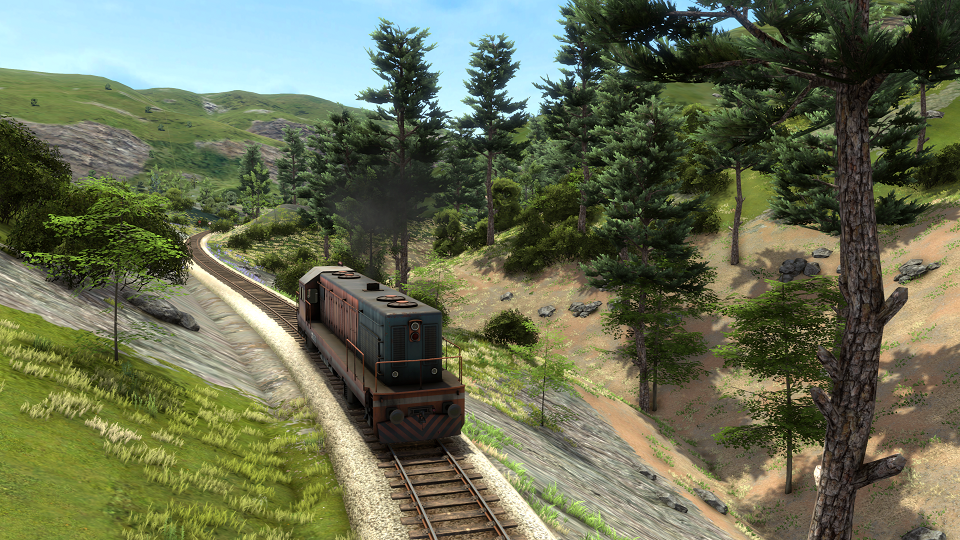
\includegraphics[width=9cm]{figures/derailvalley.png}
    %\vspace{-12pt}
    \caption{Derail Valley (Altfuture)}
\end{wrapfigure} 

Slobodan Stevic, CEO at \textit{Altfuture} and developer of \textit{Derail Valley}, explains they chose Unity “... because its VR support was better than that of other engines, back in 2016.” When asked which engine he believes is best suited for VR simulators, he adds “... it depends on the type of the simulator, its scope and style choice, as well as prior team experience.” 


\begin{wrapfigure}{l}{9cm}
    \vspace{12pt}
    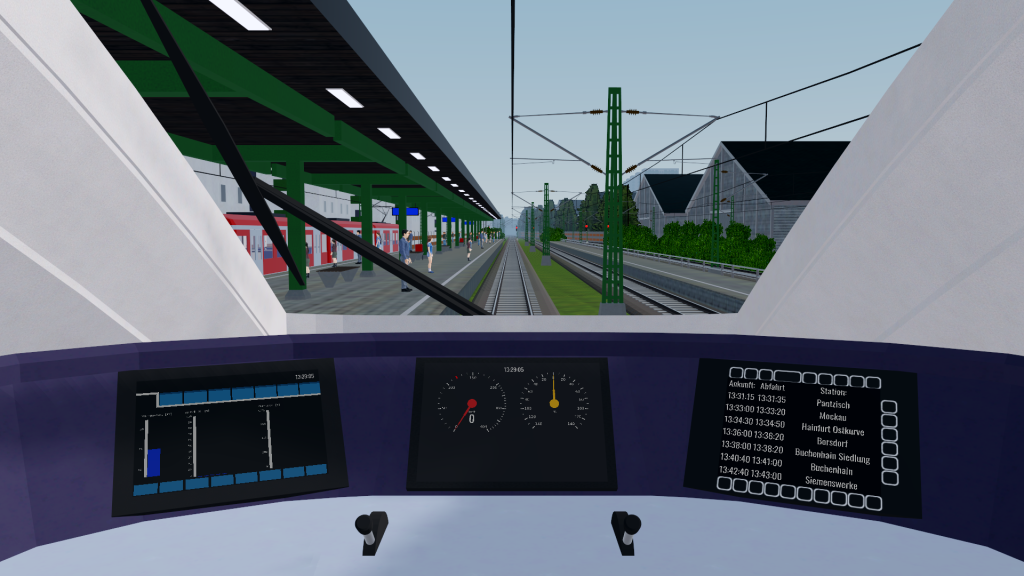
\includegraphics[width=9cm]{figures/libre_train_sim.png}
    %\vspace{-12pt}
    \caption{Libre TrainSim (GPL 3.0)}
\end{wrapfigure} 

Similarly, \textit{HaSa}, a contributor and developer of the open source project \textit{Libre TrainSim}, states that “as long as it supports `basic' requirements it is a matter of personal preference.” Describing the similarity of engine funnctioality, they also conclude that “the engine doesn't really matter.” \\[0.8cm]

Godot, the engine used to make Libre TrainSim, gets praised by HaSa for its agility. “Iteration speed is key to a good game in general. The more you iterate the better the result is.” They also comment on some downsides of the engine, claiming the renderer is “quite performance heavy out of the box which limits the creative freedom”, and the audio tools are `basic'. “We have to develop a lot of features on top to achieve good quality,” HaSa writes.

The developers we contacted behind CryEngine's small list of titles relevant to this analysis were unavailable for comment. When asking all subjects if they, in retrospect, believe their respective engine was the right choice for their game, everyone answered \textbf{yes}. 

 













%%%                 Conclusion                  %%%
\subsubsection{Conclusion}
All engines, excluding Open 3D Engine, fulfills the Absolute Requirements (\ref{absoluterequirements}) set by Lokførerskolen. Godot and Unreal supports \texttt{gltf}-files, the most prioritized asset type. Meanwhile, CryEngine and Unity are at a disadvantage as they support fewer and less prioritized assets. While all engines require a conversion pipeline for assets, Unreal and Godot can reuse more assets out of the box. This decreases time spent on porting assets to the new engine.


The overall learning curve for the individual game engines sets Unity and Unreal engine apart from the competitors. The magnitude of the community and related quantity of available material, together with their emphasis on standards in documentation, establishes their strong position in today's game engine market. Godot is still a relatively new engine without any major titles, causing both documentation and community resources to be inadequate in quality and quantity compared to Unreal and Unity. CryEngine initially limited its use to enterprise only, resulting in less publicly available resources and documentation.

The majority of developers we reached out to advocated the choice of engine to depend on the use case of the project. As such we recommended Lokførerskolen to use Unreal Engine for their train simulator. Unreal Engine has features such as a built in dedicated spline tool which we ended up basing our whole train tracks system off, as well as dynamic occlusion culling to boost performance. It also has a one of the biggest communities among the engines analysed, as well as it is known for having photo-realistic graphics. Although finding the right solution to our problems was often an issue. We found that the community is split between using blueprints or C++, and often found that blueprints were most commonly used for beginners which slowed us down in the beginning. Since we started using blueprints first to prototype or solutions, and then later on converted it to C++ code.


\section{The Product}
DeskSimV2 as a product is a functional simulator and a building tool for the simulator. The following section will provide a representation of both the simulator and the building tool.

The log in screen displays a basic user interface where the user will use their credentials to log in and gain access to the simulator. \\
\bigskip
\begin{figure}[H]
    \centering
    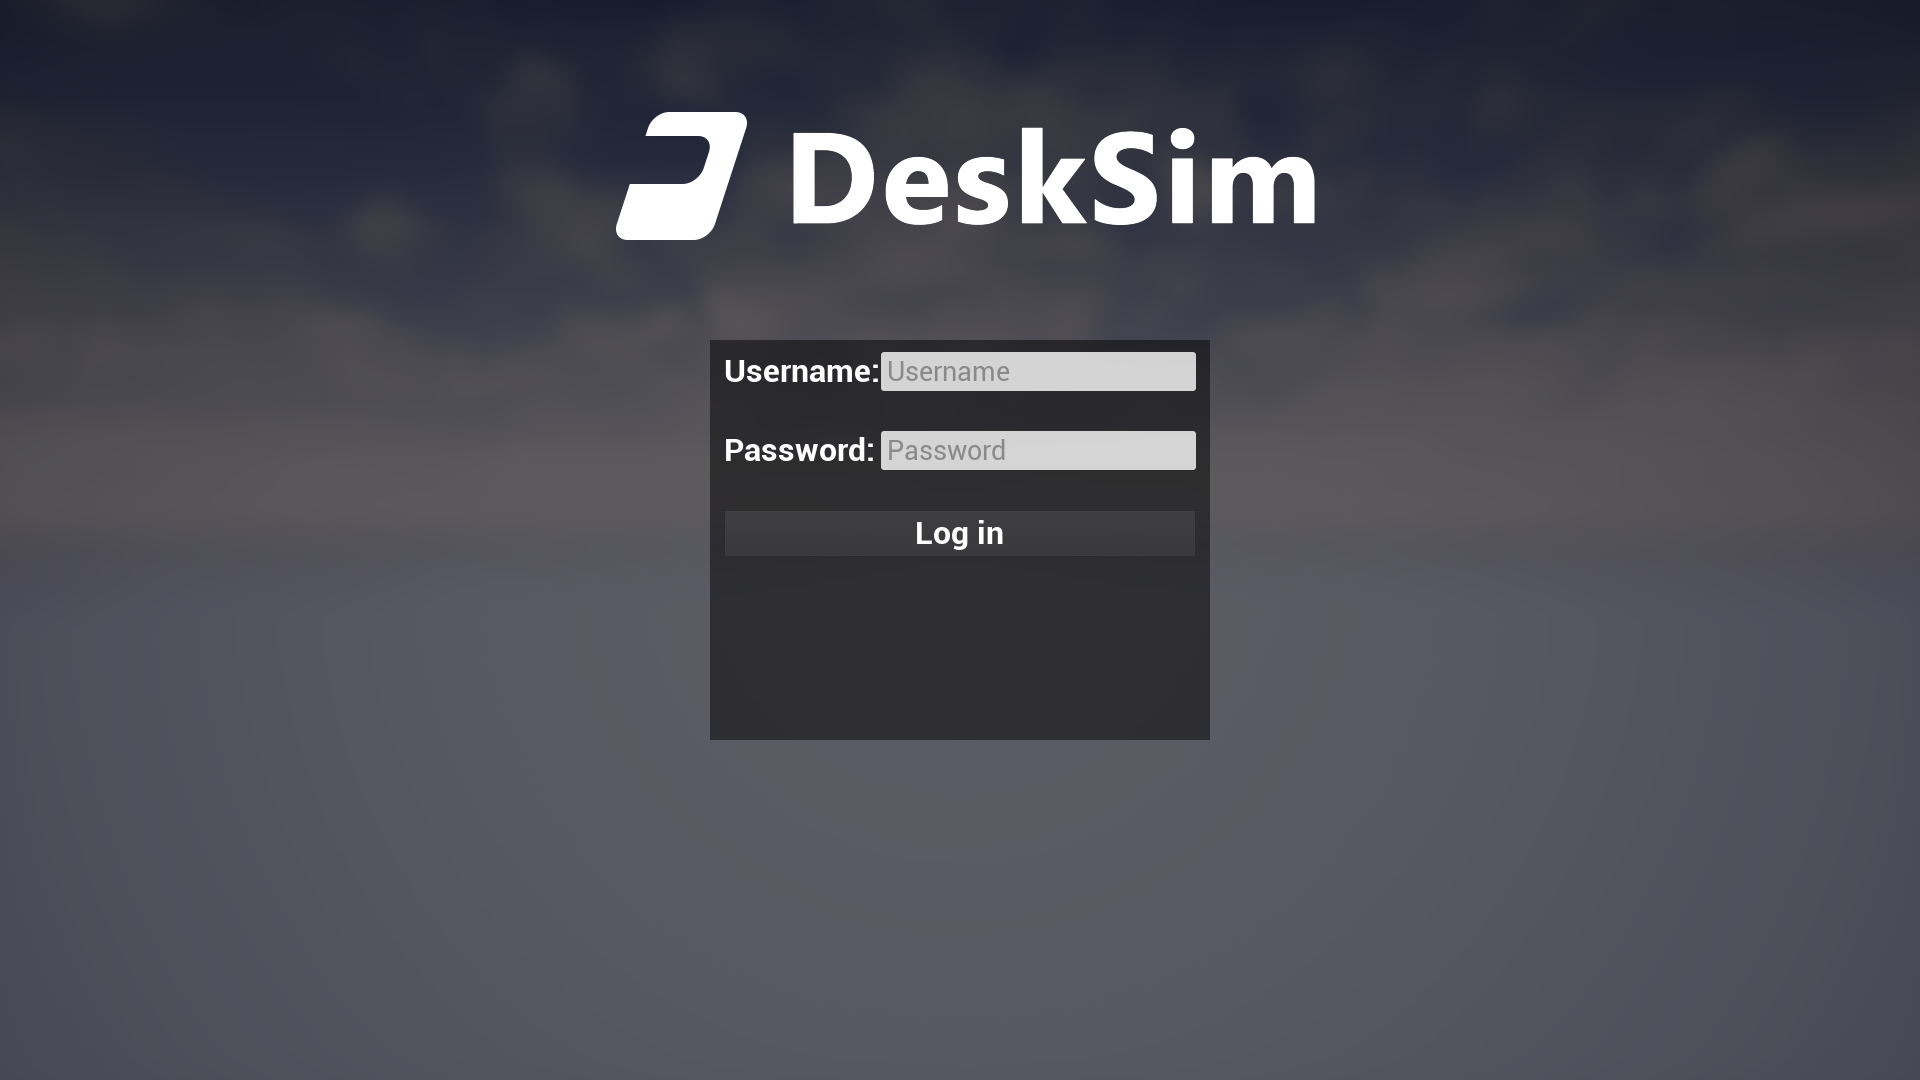
\includegraphics[width=8cm]{figures/LogIn.PNG}
    \caption{DeskSimV2: Log in Screen}
    \label{Log_in_menu_img}
\end{figure} 
\bigskip \bigskip
The main menu allows the user to select the level/scenario they want to run.
If the user has admin or teacher privileges they have the option to start a level/scenario in editing mode as well. This is shown as the "Editor" button in figure \ref{Main_Menu_img}. \\
\bigskip
\begin{figure}[H]
    \centering
    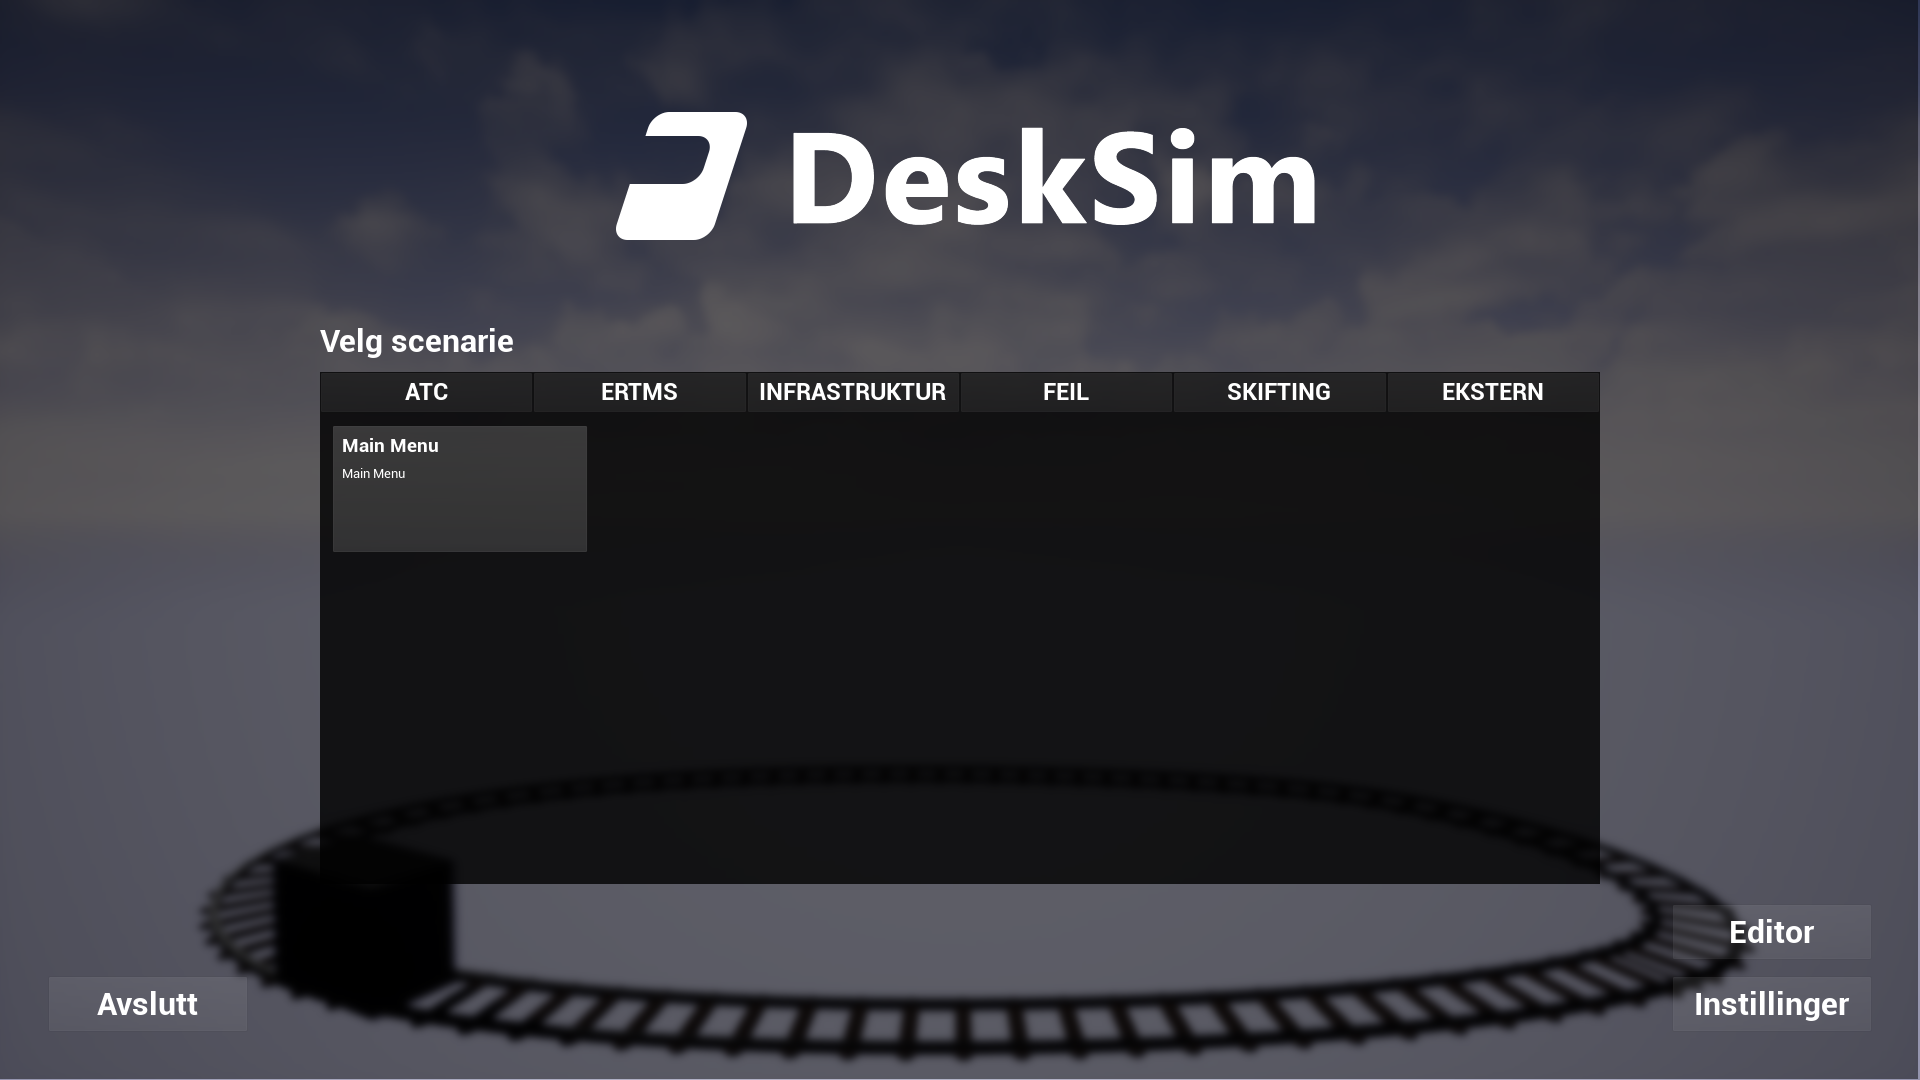
\includegraphics[width=8cm]{figures/Main Menu.PNG}
    \vspace{12pt}
    \caption{DeskSimV2: Main Menu}
    \label{Main_Menu_img}
\end{figure} 
\bigskip \bigskip
The settings menu allows the user to change the resolution and the window mode for the application
\bigskip
\begin{figure}[H]
    \centering
    \vspace{12pt}
    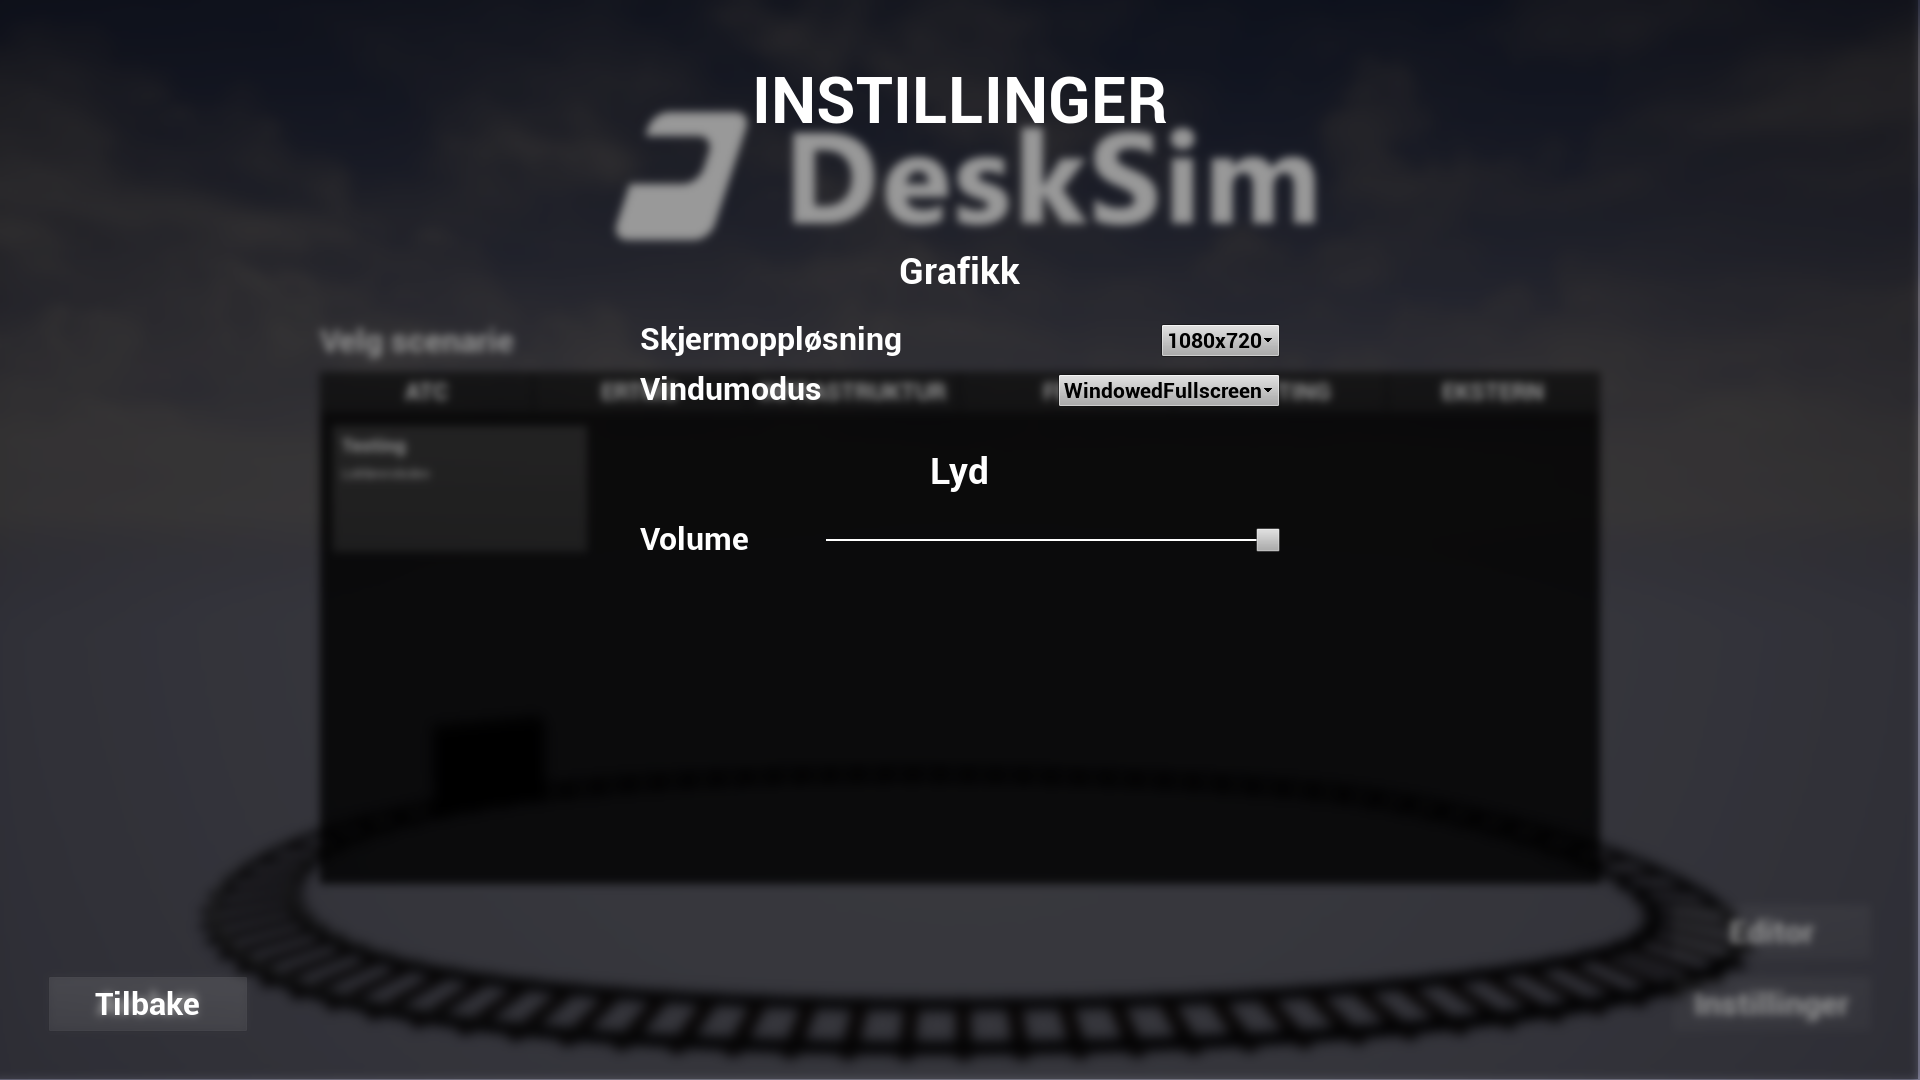
\includegraphics[width=8cm]{figures/Settings.PNG}
    %\vspace{-12pt}
    \caption{DeskSimV2: Settings Menu}
    \label{Settings_img}
\end{figure} 

The in-game experience consist of a view that corresponds to the view a train driver has from inside the front wagon of a train.
\bigskip
\begin{figure}[H]
    \centering
    \vspace{12pt}
    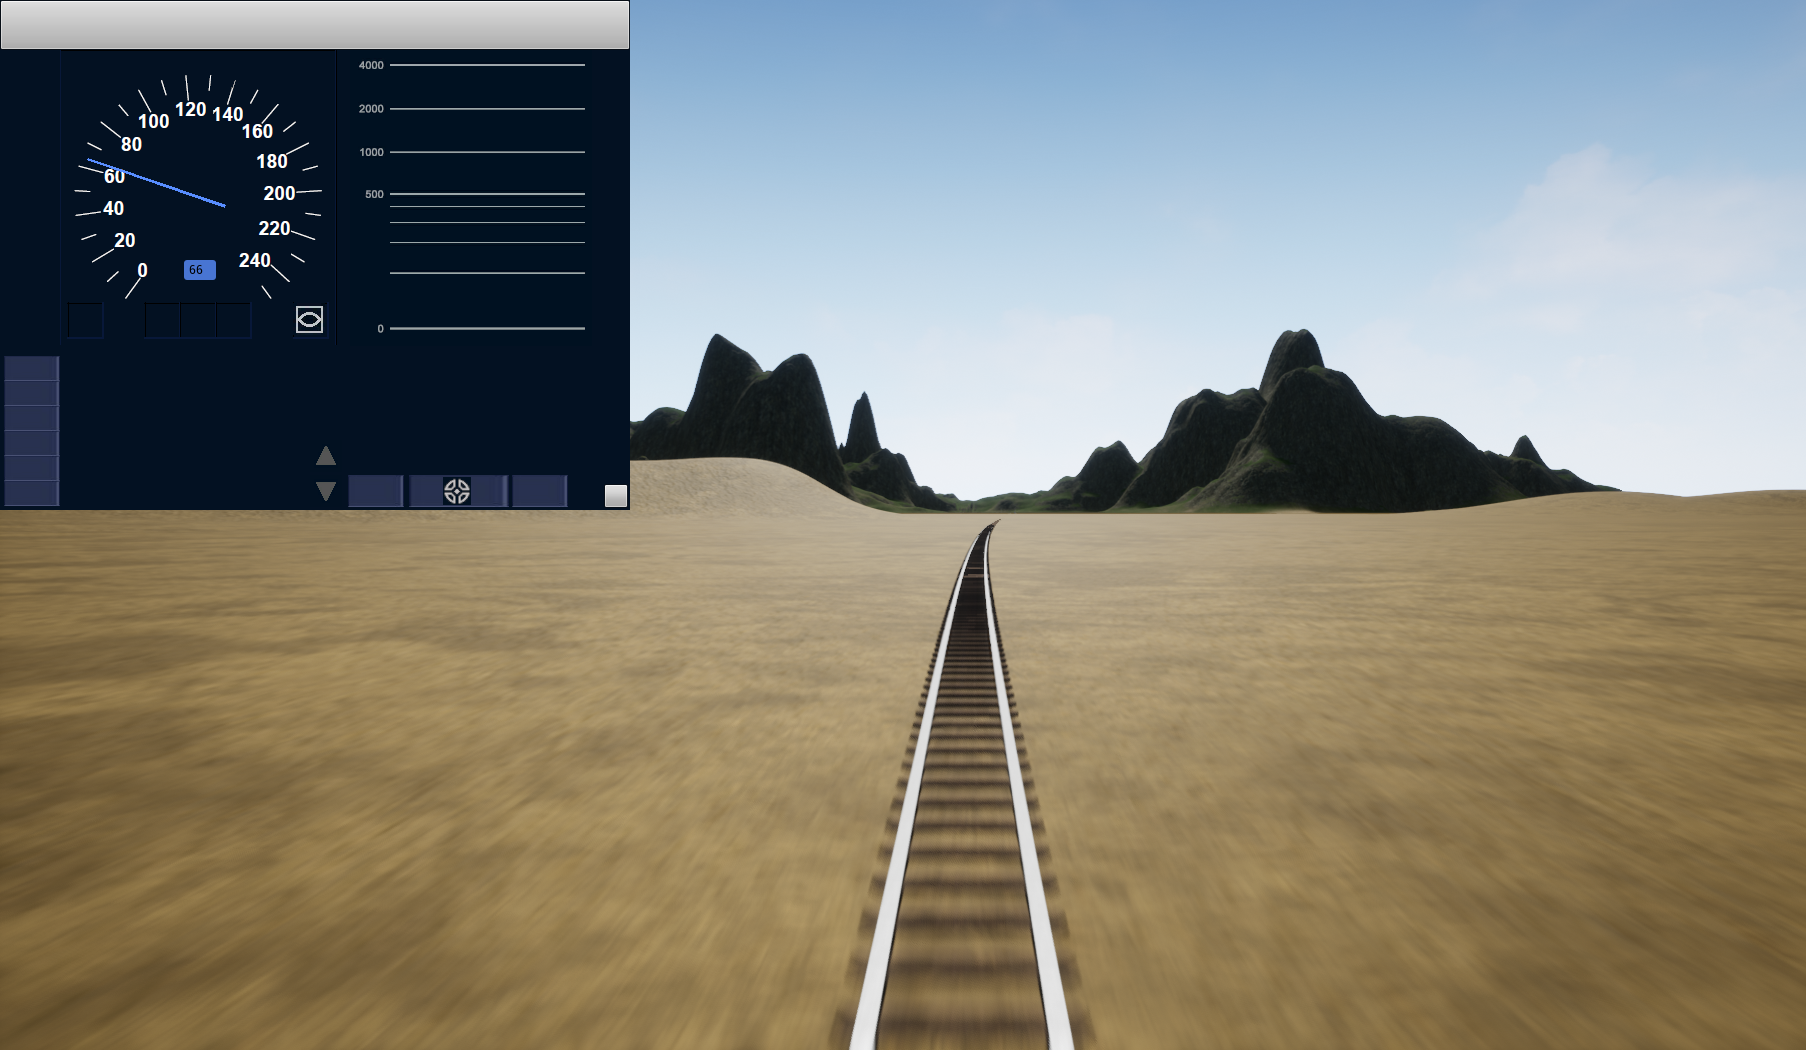
\includegraphics[width=8cm]{figures/Tog Drive.PNG}
    %\vspace{-12pt}
    \caption{DeskSimV2: Train Driver View}
    \label{Train_Driver_View_img}
\end{figure}
\bigskip \bigskip

The user will encounter different signals when running a level/scenario. The signal status and logic are predecided controlled through invisible triggerboxes and logic. 


\begin{figure}[H]
    \centering
    \vspace{12pt}
    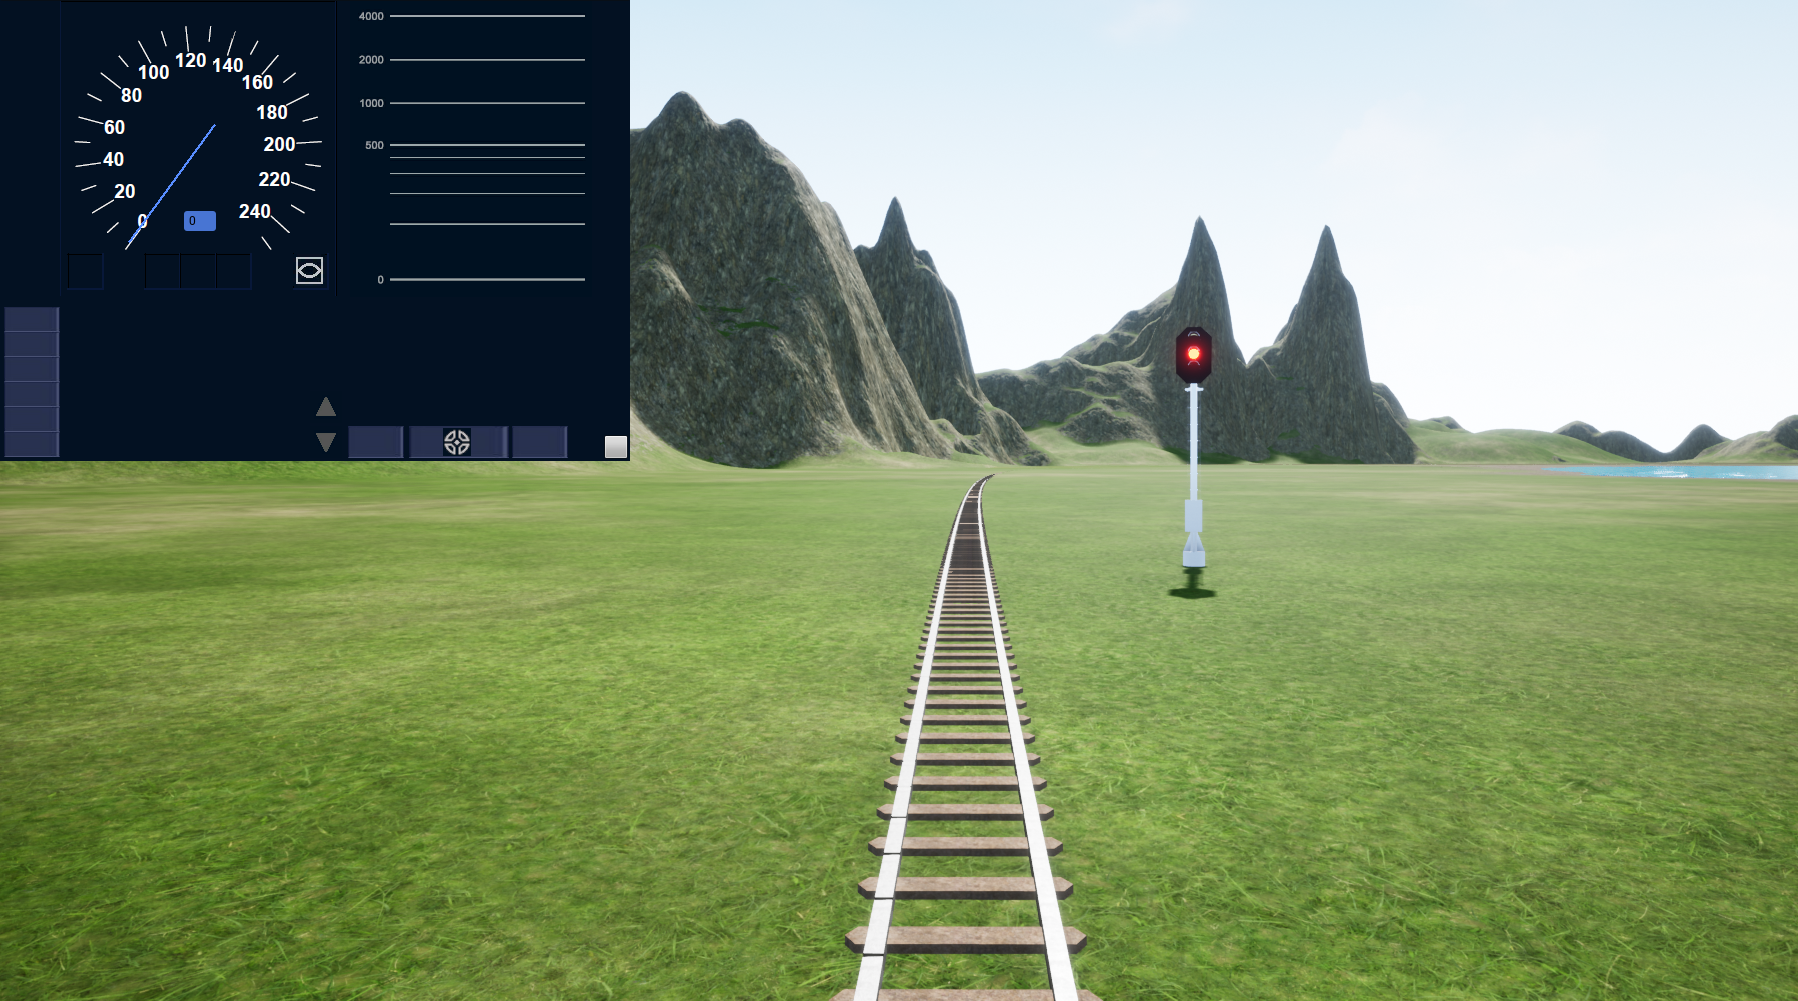
\includegraphics[width=6cm]{figures/Signal stop.PNG}
    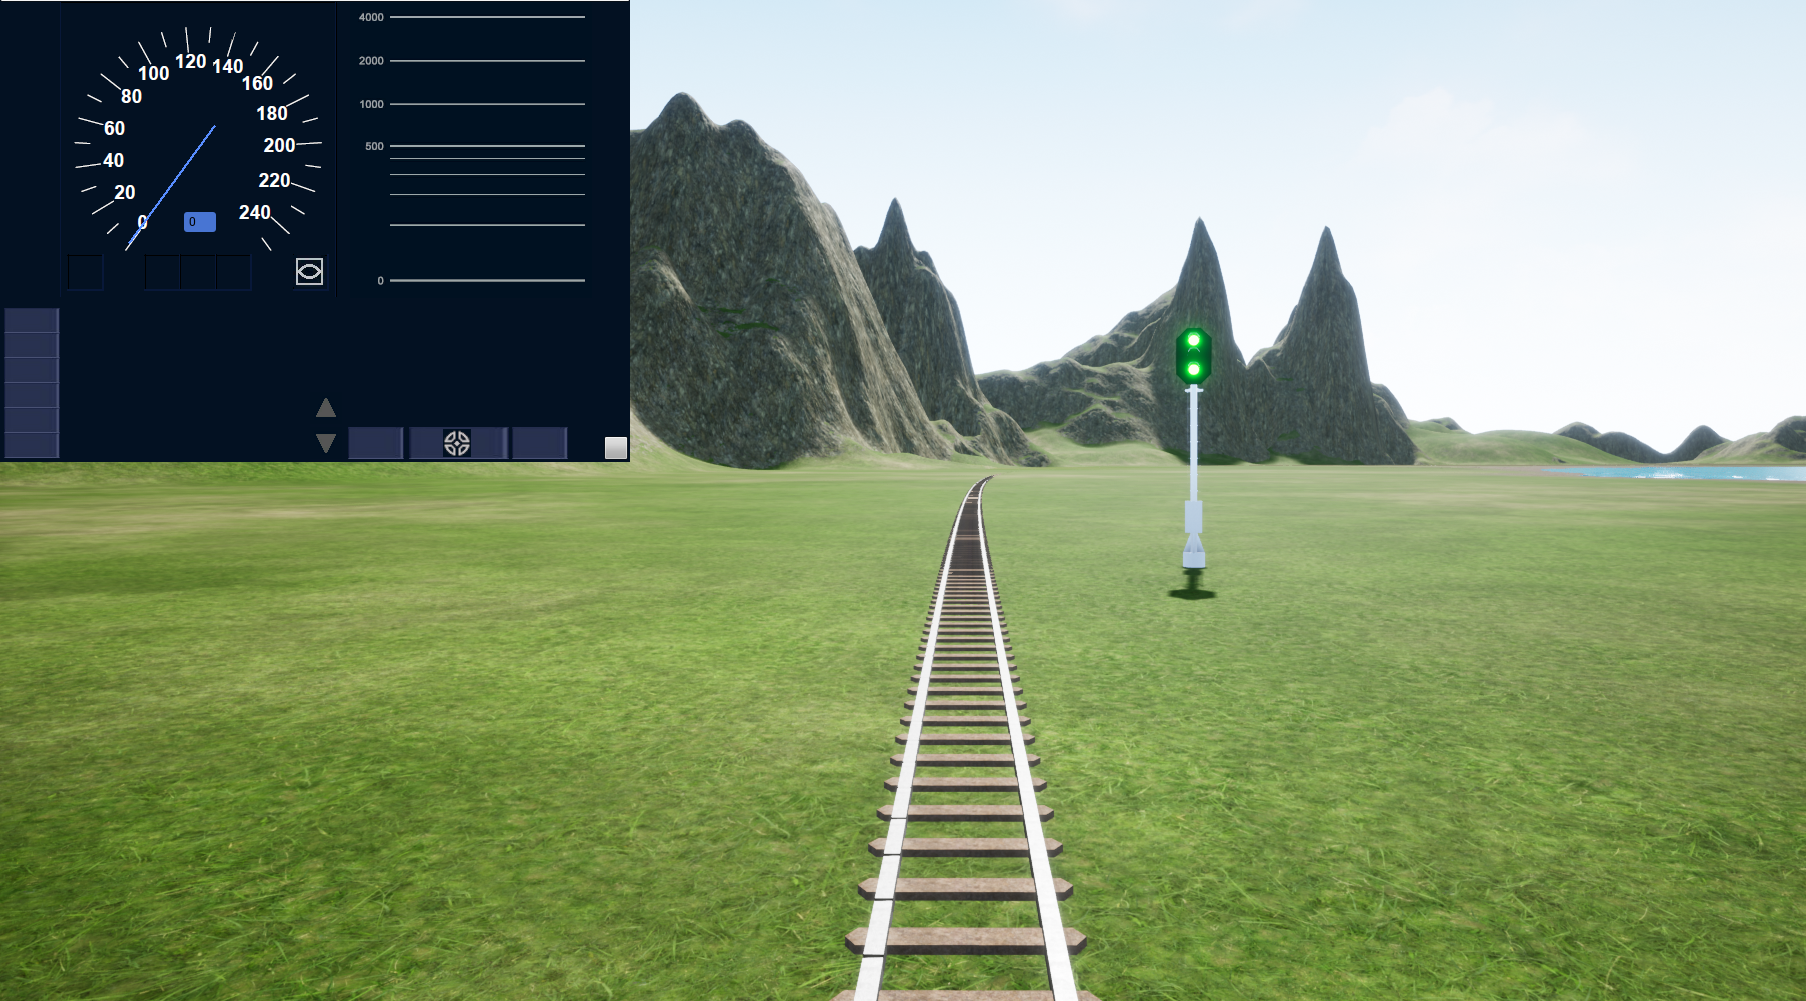
\includegraphics[width=6cm]{figures/SignalStartcorr.png}
    %\vspace{-12pt}
    \caption{DeskSimV2: Stop Signal}
    \label{Stop_Signal_img}
\end{figure} 
\bigskip \bigskip

The simulator provides an option to the user to see the world in a drone mode.
\bigskip
\begin{figure}[H]
    \centering
    \vspace{12pt}
    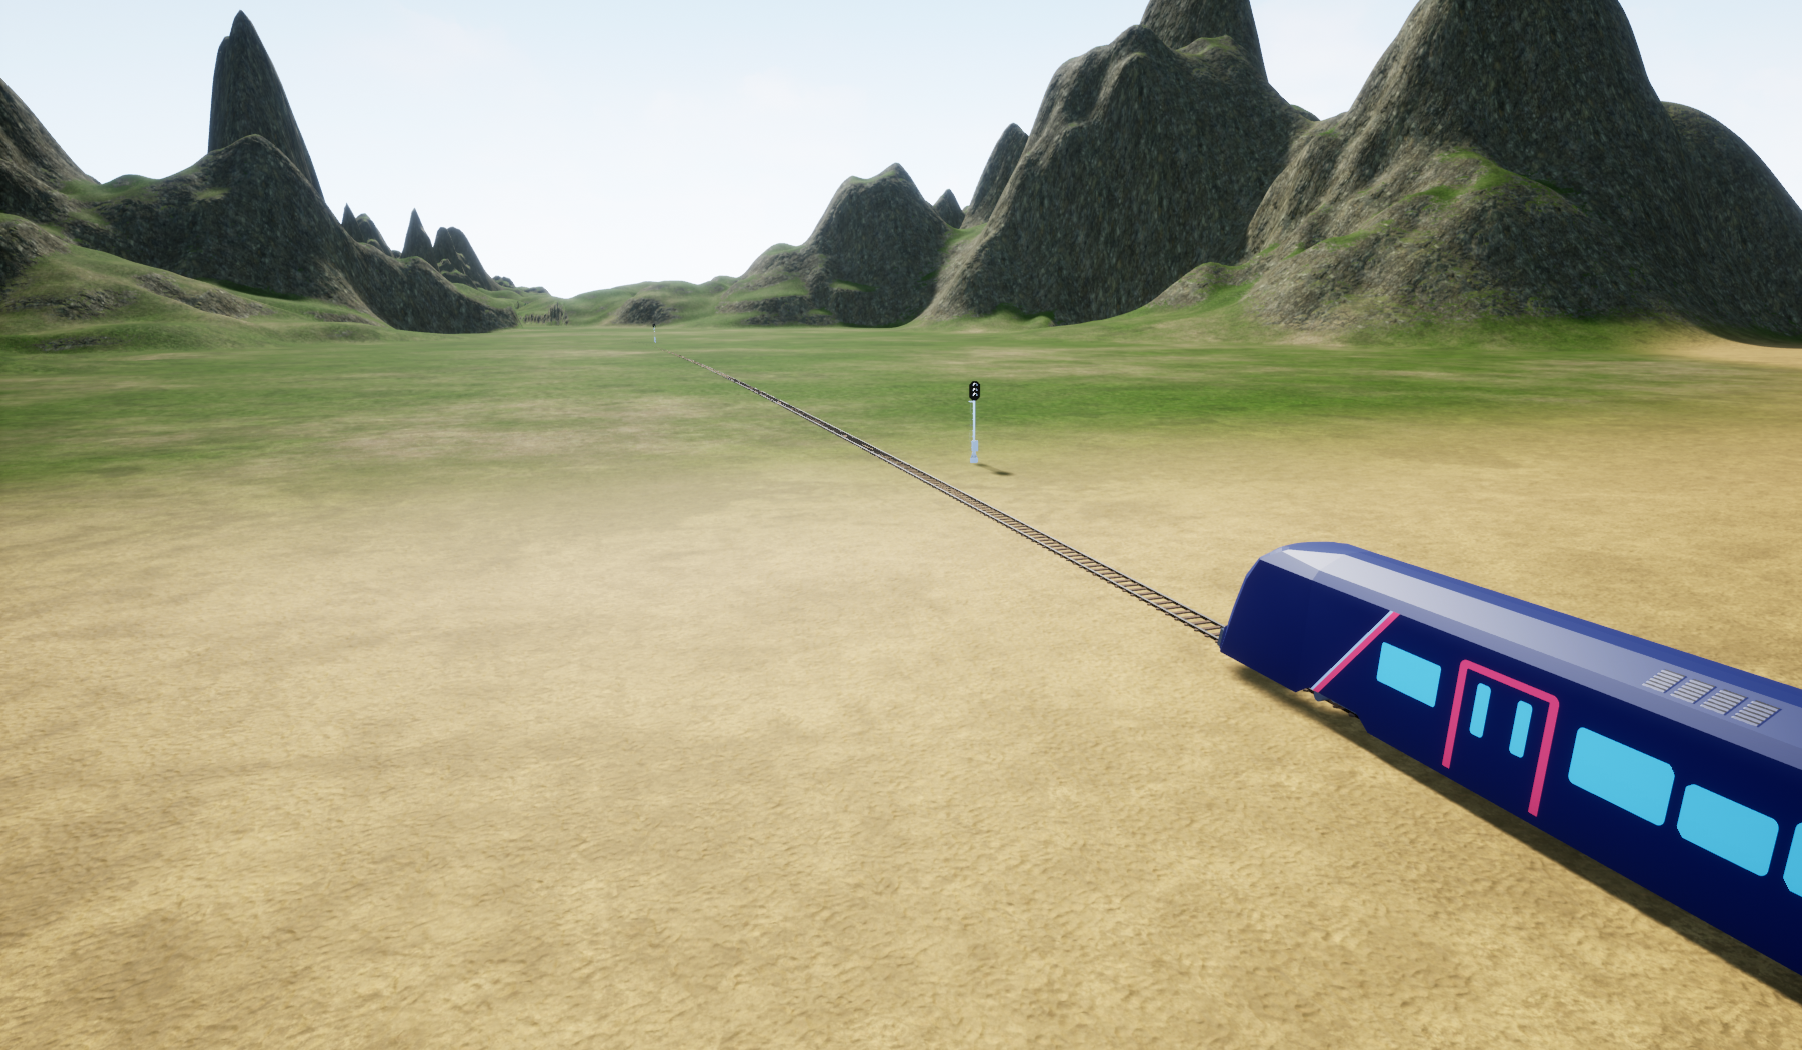
\includegraphics[width=6cm]{figures/DroneMode.PNG}
    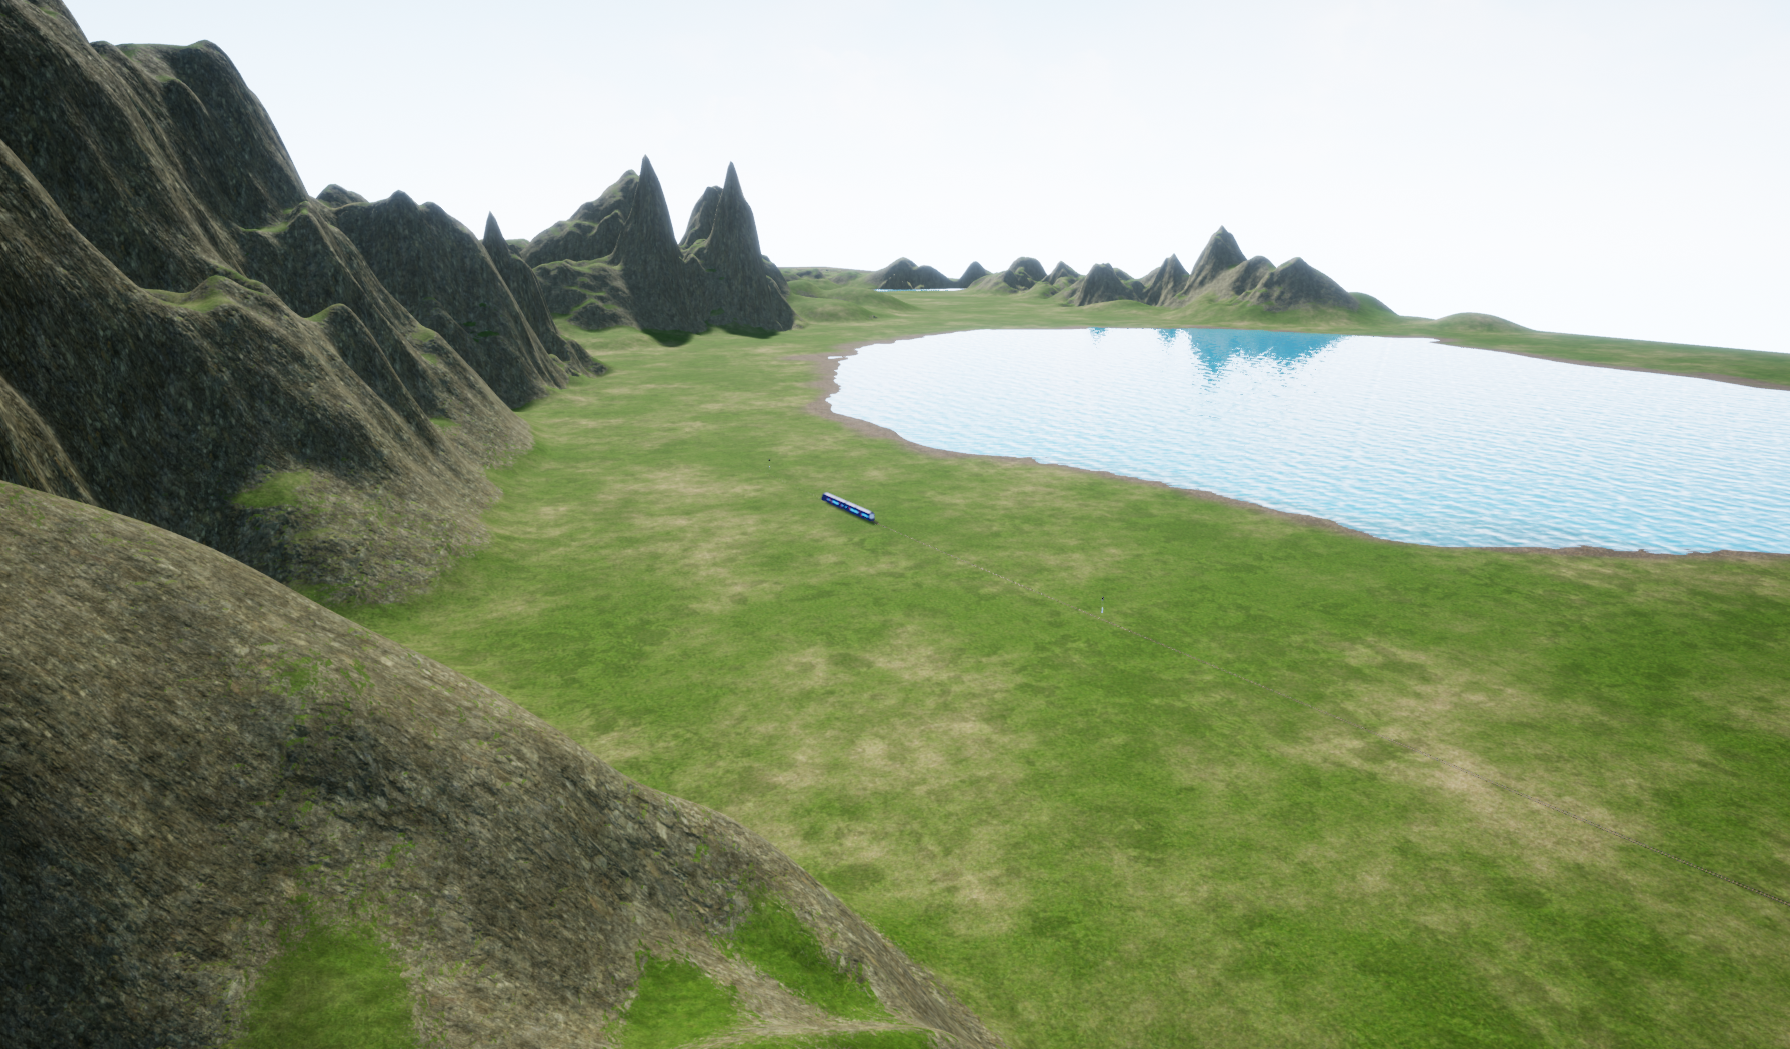
\includegraphics[width=6cm]{figures/DroneMode2.PNG}
    %\vspace{-12pt}
    \caption{DeskSimV2: Drone View}
    \label{Drone_Mode_img}
\end{figure} 
\bigskip \bigskip

The editor mode consists of a topbar where you can save your changes, change the tool mode used for objects and a trash symbol for removing objects. The other part of the User interface is the content browser where the user can drag and drop items into the level.
\bigskip
\begin{figure}[H]
    \centering
    \vspace{12pt}
    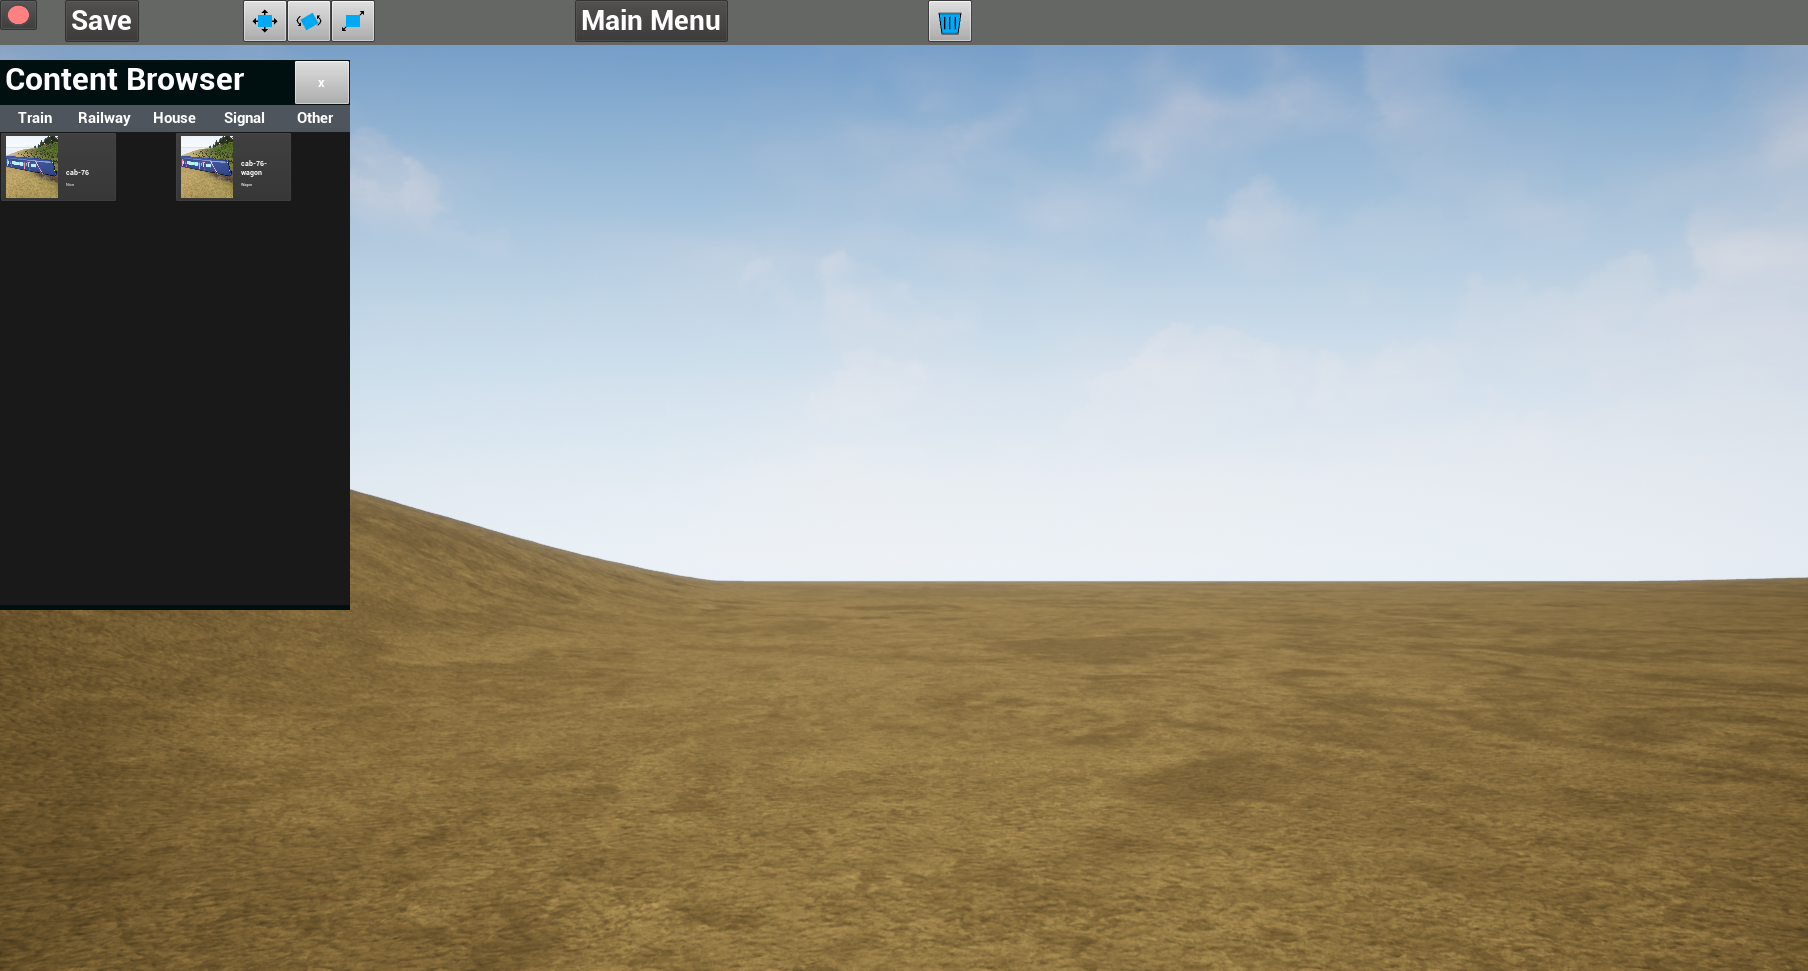
\includegraphics[width=6cm]{figures/Editor_Mode.PNG}
    %\vspace{-12pt}
    \caption{DeskSimV2: Editor Mode}
    \label{Editor_Mode_img}
\end{figure} 

\subsection{Core Functionalities}

\subsection{Menus and ui}
\section{Requirement specification}
The client stated their initial requirements in the form of one main goal and two sub-goals. The main goal included creating a demo which satisfies their requirements. They also presented two sub-goals which is a in game model placing tool and in game railway builder. Our requirement document are based on thees requirements, but does also extends further.


\subsection{Functional Requirements}
To display and visualize the core functionalities of our simulator we have chosen to utilize use cases. Use cases provides a structure and overview of the functionality works as a tool to force awareness for the requirements in the development phase. 


\subsection{Use Cases}
There was a quite unanticipated issue with defining use cases for the project as an entirety. Our main goal is, as stated previously to make a demo in the chosen engine and also make the code applicable for further development. What we discovered in the development of the demo was that the classes and structures we created often layed a groundwork for further development. We therefore decided to include two separate groups of use cases for our project. One for the application it self, and one for the use cases that got facilitated by us through development. The reasoning for including this is for the client to more easily understand the functionality and it requires us to focus on the code quality and further development perspective of the project.

\subsection{Use Case Diagram: Application}
The use case diagram illustrates all available actions for the two groups of users; students and employees. To avoid cluttering, it is implied that an employee has access to all functionality of the student.
\begin{figure}[H]
\centerline{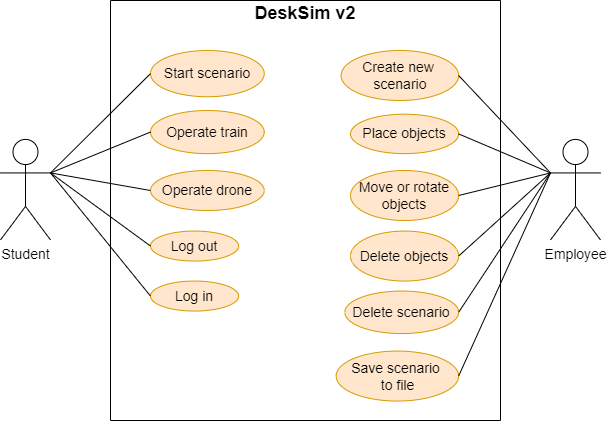
\includegraphics[width=1.0\textwidth]{figures/UseCaseDiagramApplication.png}}
\caption[size=small]{Use case diagram - Application}
\label{use_case_engine}
\end{figure} 

\subsubsection{High Level Use Case}

% CREATE NEW SCENARIO
\begin{table}[H]
    \centering
    \begin{tblr}{colspec={|X[.2, l]|X[.8, l]|}, hlines}
        \textbf{Use Case:} & Create new scenario \\
        \textbf{Actors:} & Employee \\
        \textbf{Goal:} & To create, build and save a new scenario \\
        \textbf{Description:} & The user clicks at the "New Scenario" button in the main menu to open up an editor screen. From here, the user can freely define the start point, curvature, and end of a railway path. The user can also drag objects like signals or buildings into the scenario. Finally, the user can save the scenario to a file, making it playable from the main menu. \\
    \end{tblr}
    \caption{Use Case: Create new scenario}
\end{table}

\vspace*{1 cm} %Temporary fix for tables going into eachother

% PLACE OBJECTS
\begin{table}[H]
    \centering
    \begin{tblr}{colspec={|X[.2, l]|X[.8, l]|}, hlines}
        \textbf{Use Case:} & Place objects \\
        \textbf{Actors:} & Employee \\
        \textbf{Goal:} & To place the necessary objects such as a train and a railway in a level. \\
        \textbf{Description:} & When a level is opened in editor mode the user is provided a user interface which includes a content browser. The user can click on a item in the content browser and drag it out in the level. The content browser has different categories the user can select in the top bar by clicking on the category buttons.
    \end{tblr}
    \caption{Use Case: Place objects}
\end{table}

\vspace*{1 cm} %Temporary fix for tables going into eachother

% DELETE OBJECTS

\begin{table}[H]
    \centering
    \begin{tblr}{colspec={|X[.2, l]|X[.8, l]|}, hlines}
        \textbf{Use Case:} & Delete objects \\
        \textbf{Actors:} & Employee \\
        \textbf{Goal:} & To delete an object in the level. \\
        \textbf{Description:} & When clicking on an object in a level the user will be given the option to remove it. After the click, the user will get a trash can symbol at the top bar, next to the transformation options. After clicking on the trash can, the program will prompt the user for confirmation before permanently removing the object from the scene.
    \end{tblr}
    \caption{Use Case: Delete objects}
\end{table}

\vspace*{1 cm} %Temporary fix for tables going into eachother

% OPERATE DRONE
\begin{table}[H]
    \centering
    \begin{tblr}{colspec={|X[.2, l]|X[.8, l]|}, hlines}
        \textbf{Use Case:} & Operate drone \\
        \textbf{Actors:} & Student \\
        \textbf{Goal:} & Maneuver the drone camera \\
        \textbf{Description:} & When the student clicks the drone view button "2", the student can freely move around in the scenario using W, A, S and D for forwards, backwards and horizontal movement, Q for downward and E for upward movement. The user can also use the mouse to freely look around in the scenario, and change the movement speed with the scroll wheel.
    \end{tblr}
    \caption{Use Case: Move or rotate objects}
\end{table}


\subsubsection{Low Level Use Case}

% NEW, move or rotate object
\begin{table}[H]
    \centering
    \begin{tblr}{colspec={|X[.2, l]|X[.8, l]|}, hlines}
        \textbf{Use Case:} & Move or rotate objects \\
        \textbf{Actors:} & Employee \\
        \textbf{Goal:} & To move a object or rotate it into the prosition and position you want \\
        \textbf{Precondition:} & The user has successfully opened a scenario in editor-mode \\
        \textbf{Success Scenario:} & 
        
            1. The employee clicks on the object he wants to edit. \newline
            2. The object will display a gizmo, either in the form of arrows the move it along either it's x, y or z axis, or a wheel to rotate. \newline
            3. The user changes the mode to the one he want from the top bar icons. \newline
            
            4. \textbf{For translation:}\newline
                5. The user hovers the mouse over the gizmo arrow to select one axis, or in the middle of two  gizmos to select a plane and presses the gizmo. \newline
                6. The user drags the mouse to the position he wants the object to be located \newline
                
            4. \textbf{For rotation:} \newline
               5. The user presses the wheel and drags the mouse around the wheel to get the desired rotation. 
    \end{tblr}
    \caption{Use Case: Move or rotate object}
\end{table}

\begin{table}[H]
    \centering
    \begin{tblr}{colspec={|X[.2, l]|X[.8, l]|}, hlines}
        \textbf{Use Case:} & Operate Train \\
        \textbf{Actors:} & Student \\
        \textbf{Goal:} & To drive the train in a scenario \\
        \textbf{Precondition:} & The user has successfully opened a level and the levers is connected to the system through a USB port \\
        \textbf{Success Scenario:} & 
            1. The user pushes the left lever or "w" key to accelerate the train. \newline
            2. The user pushes the right lever to apply break force on the train. \newline
            3. Depending on the scenario, the user has to follow some rules: \newline


                The user should not exceed the speed limit. Doing so should result in system regulated brakes turned on. \newline
                
                The user is provided information about the current speed in the Driver Machine Interface. \newline
                
                The user should follow the rules regulated by signals: \newline


                    \textbf{Main signal:} If this signal is red the user should stop. If user don't stop before the signal this should result in breaks turned on.
                    
                    \textbf{Main signal:} One green light means that the user can drive with reduced speed.
                    
                    \textbf{Main signal:} Two green lights means that the user can and should continue with the set speed.

    \end{tblr}
    \caption{Use Case: Operate Train}
\end{table}

\subsection{Use Case Diagram - Game engine}


\begin{figure}[H]
\centerline{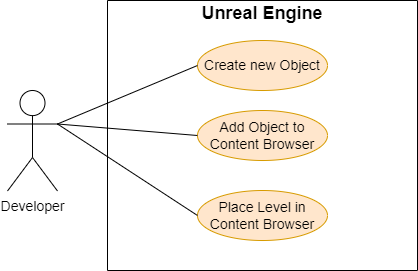
\includegraphics[width=1.0\textwidth]{figures/UseCaseDiagramGameEngine.png}}
\caption[size=small]{Use case diagram - Game Engine}
\label{use_case_application}
\end{figure} 

\subsubsection{High Level Use Case}

\begin{table}[H]
    \centering
    \begin{tblr}{colspec={|X[.2, l]|X[.8, l]|}, hlines}
        \textbf{Use Case:} & Add Level in Main Menu \\
        \textbf{Actors:} & Developer \\
        \textbf{Goal:} & To add a level created in unreal engine to the simulator.. \\
        \textbf{Description:} & When the developer has created a scene he wants to be a part of the simulator he must know the name of the level. The level name is stored as a FName, and the content browser only need its value. The FName's are immutable and case sensitive so it's important to have the right name. Open the MMObjects inside \textit{BP\_EditorHUD} blueprint located in "\textit{DeskSimV2/Source/DeskSimV2/Editor/UI}". The developer now clicks the + button to add the new level and fills in the name, description and the FName reference to the map. 
    \end{tblr}
    \caption{Use Case: Add Level in Main Menu}
\end{table}


\subsubsection{Low Level Use Case}


\begin{table}[H]
    \centering
    \begin{tblr}{colspec={|X[.2, l]|X[.8, l]|}, hlines}
        \textbf{Use Case:} & Add new object \\
        \textbf{Actors:} & Developer \\
        \textbf{Goal:} & To add a new object to the game \\
        \textbf{Preconditions:} & The developer has a working version of Unreal Engine version 4.27.2 or higher. The developer has a 3D model he wants to be added in the game.  \\
        \textbf{Success Scenario:} & 

            1. The developer uploads the model to the "models" folder inside unreal engine \newline
            2. The developer navigates to "C++ classes" in the content browser. \newline
            3. The developer right clicks on either "BasicStaticObject", "Train" or "BasicSignal" or "wagon", based on what item type the object is.\newline
            4. The developer clicks on "Derive blueprint from c++ class..." in the drop-down menu and selects the appropriate place to store the blueprint.\newline
            5. The developer opens the blueprint and drags the imported model from step 1 into the "Static mesh" variable in the details panel for the object.\newline
            6. The developer compiles and saves the blueprint \newline

    \end{tblr}
    \caption{Use Case: Add new object}
\end{table}

\begin{table}[H]
    \centering
    \begin{tblr}{colspec={|X[.2, l]|X[.8, l]|}, hlines}
        \textbf{Use Case:} & Add object in Content Browser \\
        \textbf{Actors:} & Developer \\
        \textbf{Goal:} & To successfully add a created object in the content browser making it clickable and draggable in runtime.\\
        \textbf{Preconditions:} & The developer has created a new object as described in the "Add new object" use case.  \\
        \textbf{Success Scenario:} & 

            1. The developer open the \textit{BP\_EditorHUD} blueprint located in "\textit{DeskSimV2/Source/DeskSimV2/Editor/UI}". \newline
            2. The developer clicks on the \texttt{+} icon for the CBFObjects. \newline
            3. The developer adds the category the actor should be a part of.\newline
            4. The developer writes a suitable name and description for the object. \newline
            5. The developer adds the reference to the actor he wants to include.\newline
            
            6. Close unreal engine desktop and visual studios and navigate to the file system for the project. Right-click on the \textit{DeskSimV2.uproject} files and select "generate visual studios project files" from the dropdown menu.\newline
            7. The item should be visible and draggable in-game in the content browser. \\
        
        \textbf{Alternative Scenario:} & 
        
            6. Open visual studio and right click on DeskSimV2, select "rebuild" and let the solution rebuild. \newline
            7. When its built, open DeskSimV2.uproject and check if the object is added.

    \end{tblr}
    \caption{Use Case: Add object in Content Browser}
\end{table}

\vspace*{1 cm} %Temporary fix for tables going into eachother

\subsection{Operational Requirements}
These are the requirements which concerns the application at it's operational stage, this stage begins at the project's deadline which is the 20.th of May:
\begin{itemize}
    \item The application must be able to interact with the existing Rest-API hosted by Lokførerskolen.
    \item The system must operate on Windows devices.
    \item The system must manage privileges of users and only allow elevated users to access the editor functionality.
    \item Must be transferable through a zip file
    \item The system must operate on computers which has 8GB of ram and a Intel® Core™ i5-4460 CPU or better. 
    \item Should not experience frame rate drops of lover than 60 frames per second. 
\end{itemize} 


\subsection{Security and Misuse}
To ensure the security of the users and avoid misuse of the application the application:
\begin{itemize}
    \item must require user authentication for usage. The authentication process should be a token based system where you receive a token. The token has an expiration and should be used to authenticate the user up to its expiration. When the token expires the user will be asked to authenticate again and recieve a new token. % er dette operational?
    \item should not contain bugs and/or security flaws that potentially could lead to harm or destruction of hardware components. Such flaws include bad memory handling.
    \item must not store any passwords in plain text.
\end{itemize}


\subsection{Interface Requirements}
\textbf{Menus} 
\begin{itemize}
    \item It should  be intuitive and easy for a student at Lokførerskolen to navigate the Main Menu. 
    \item The Main Menu should have the same functionality as the previous simulator and only deviate by design.
    \item All text must be available in Norwegian.
    \item Buttons should be intuitive to reduce the number of operations required for a task.
\end{itemize}

\textbf{Scenarios} 
\begin{itemize}
    \item The game should have an option to switch between A Drone Mode and a Train Mode. 
    \item The DMI viewport in a game should be responsive to the gameplay and be movable for the player.
    \item All numbers and measurements must be specified in the metric system.
\end{itemize}



\subsection{Product Backlog}


\section{Design}

\subsection{System Architecture}

The code architecture is based around the object-oriented nature of C++ and patterns within game programming. Limited by the development environment, we had to implement all classes as derivatives from Unreal Engine's base classes. These classes enable common functionality such as rendering, collisions and mathematical operations such as translation and rotation. We continued this style of inheritance, defining base properties for objects, and deriving further into special classes if needed. A prime example of this is in the editor mode of the application, where each object in a level is treated as an \textit{EditorObject}, including trains and railways. An EditorObject is an interactable entity in a level. These can be manipulated by the EditorController, which handles all user input and level manipulation.

\vspace*{1 cm} %Temporary fix for tables going into eachother

\begin{figure}[!htb]
    \centerline{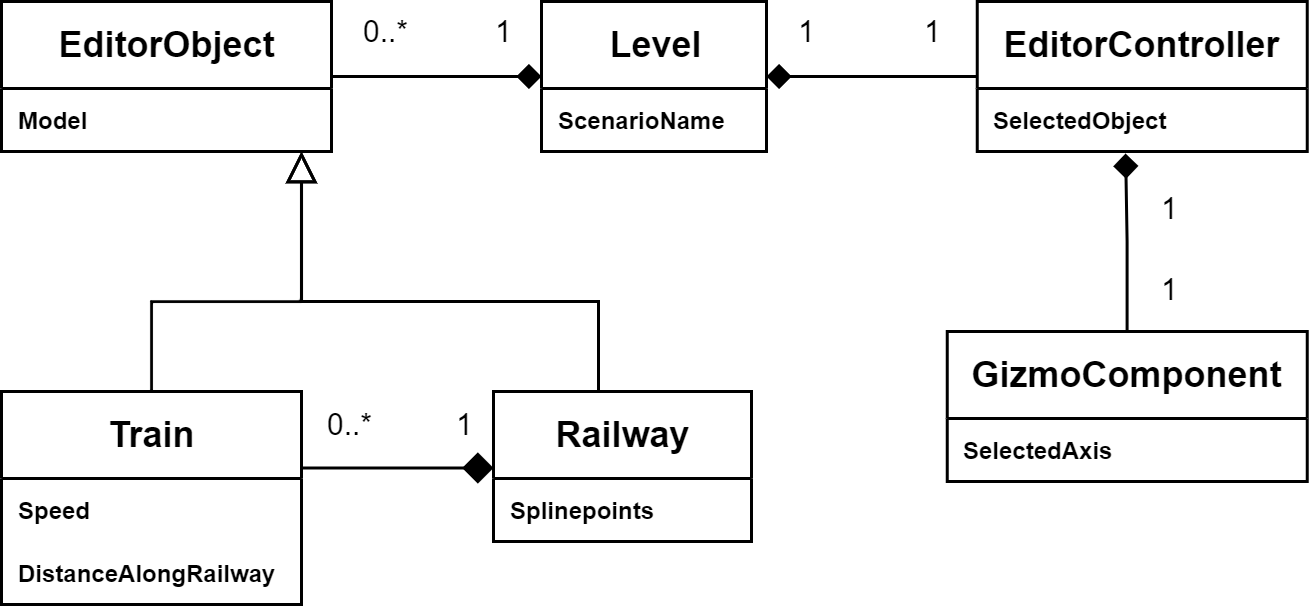
\includegraphics[width=0.9\textwidth]{figures/EditorERDiagram.png}}
    \caption[size=small]{Class diagram for the editor mode}
\end{figure} 
\vspace*{1 cm} %Temporary fix for tables going into eachother

\subsubsection{Authentication}

User authentication is done using the existing solution in use at Lokførerskolen. Their system uses two endpoints, the first receives a username and password and returns a JWT (Json Web Token) on success. The JWT is then sent to the second endpoint, which returns a JSON UserObject which contains info such as ID, Username, Roles, etc. 

When the program is launched a login screen is presented to the user, where a username and password must be entered. The user must be authenticated in order to use the software. If an error occurs, such as invalid username or password, or an error with the server, an error message is shown to the user. Once the user is authenticated their info is stored for the duration of the session. The user-info is never stored to any file, which means the user needs to log in again when the program is started again. Because the username, password nor token is ever stored locally, they cannot be extracted from local files in order to obtain private credentials.


%The system for authenticating user credentials utilizes REST-technology over HTTPS (Hypertext Transfer Protocol Secure). The authentication is done by sending a POST-request to the client's API with a username and a password formatted as a JSON object.

\vspace*{1 cm} %Temporary fix for tables going into eachother
\begin{figure}[!htb]
    \centerline{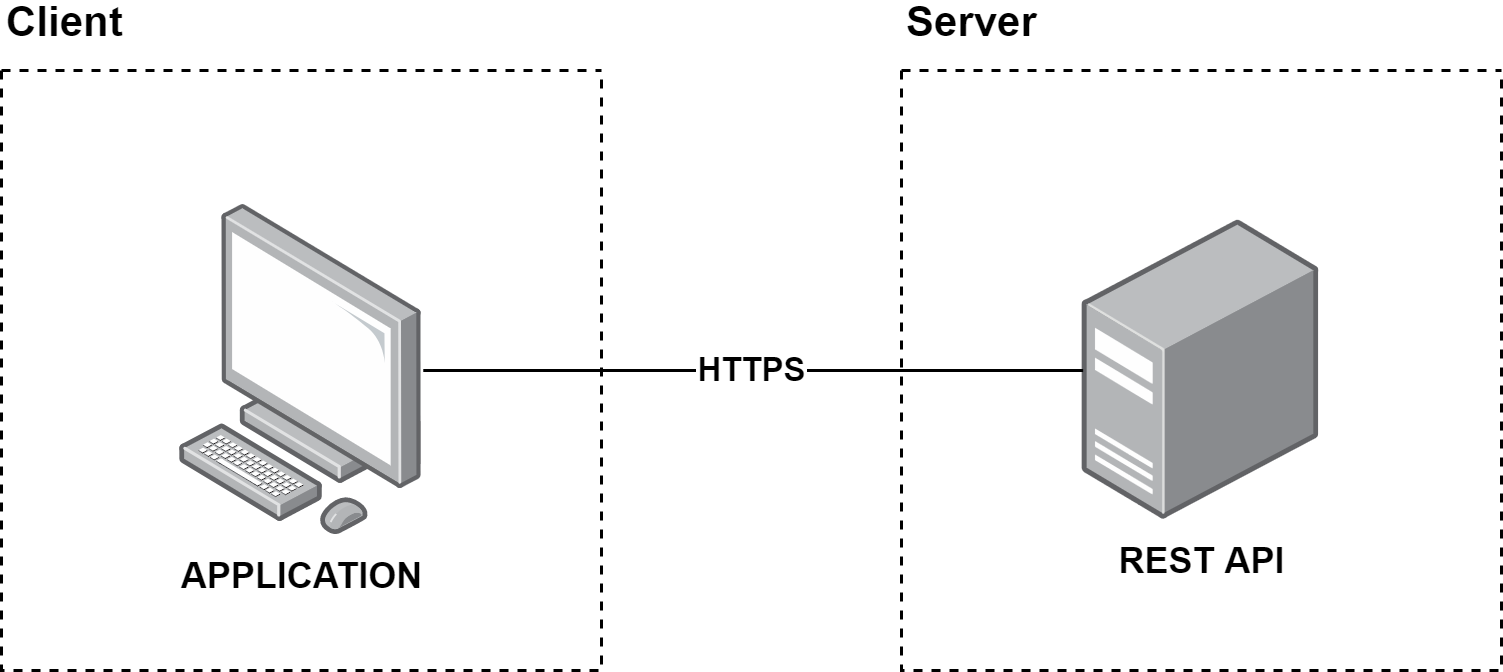
\includegraphics[width=0.9\textwidth]{figures/NetworkArchitecture.png}}
    \caption[size=small]{A diagram for the network architecture}
\end{figure} 

\subsubsection{Scenarios}
% System
\subsection{Design choices}
% 

% Have to figure out what to include in this section!

\newpage
\section{Development Process}

This chapter will provide a detailed description the methodology, and how we used it. It will describe some of our sprints and the project process as an entirety. There will also be a graphical view of the sprints showing the progress, and explanations over changes in the project scope.


\subsection{Scrum}

%% basic info about scrum?
%scrum is and agile development model, which allows for an iterative development cycle with a focus on completing work in 2-4 week long sprints. (add source here). 
%% compare canban and scrum, as they are both agile

For this project we chose to use scrum, as it allows us to quickly adapt to changing requirements. Due to the freedom given in this task this methology seamed to be the best fit. Scrum also allows us to quickly iterate on features, in order to get feedback from Lokførerskolen. 
The agile nature of scrum allows us to plan and divide the work into issues during the project. As such, we only divided work and created issues for the milestone currently in progress. This allows us to focus on the milestone at hand, without worrying about planning what to do in a future milestone where requirements or tasks might change.

In addition we have experience using scrum, as we used scrum in a previous course. Therefore we have experience with the workflows and structure used in Scrum. 

% HOW WE USED SCRUM
In the start of the project we used scrum strictly as described in the project plan[Link], where we had daily scrum meetings every day and sprint planning meetings in the beginning of each sprint. After the fourth sprint we decided to stop with the daily scrum meetings, the decision was mostly based on the value we got from the meetings. In the project planning phase we thought that the group was going to work individually and that it could be hard for everyone to keep an overview of the project. 

%% talk about jira, which we use to track sprints
In this project we used Jira for Scrum related work, such as creating sprints and to track milestones, stories, and issues. 

Jira also gives reports and graphs on the rate of work and issues created and finished during the project. 



another agile development model which we considered is canban, which is based on a board of tasks, where only a certain amount of tasks can be in progress at the same time. (add source here) 

%% code convention? process of learning unreal? 

\subsection{Methodology}

%% how we worked and our routines?

The group agreed on having workdays be from Monday to Friday, with standard work hours from 09.00 to 15.00. During this time 

workdays are mon-fri
workdays from 09.00 to 15.00 
time and days can be deviated from as needed, just notify the group

how we worked together
work from home, sit in voice chat room during workday
work is mostly solo on features, but we cooperate when merging features, working on common functionality, fixing problems or teaching each other stuff.
time tracking on jira using clockify addon, provides time tracking available for each issue


small daily meeting at the start of the day, stopped doing after a while
started with 1 week sprint length, switched to 2 weeks after main goal mvp was done
sprint meeting at start of week, group discusses progress and what issues to include in the next sprint

supervisor meetings
client meetings
retrospective meetings \& ... meetings 

%%%%%%%%%%%%%%%%%%%%%%%%%%%%%%%%%%%% SCRUM %%%%%%%%%%%%%%%%%%%%%%%%%%%%%%%%%%%%%%%%%%

\subsection{Sprints}

\begin{figure}[H]
    \centering
    \vspace{12pt}
    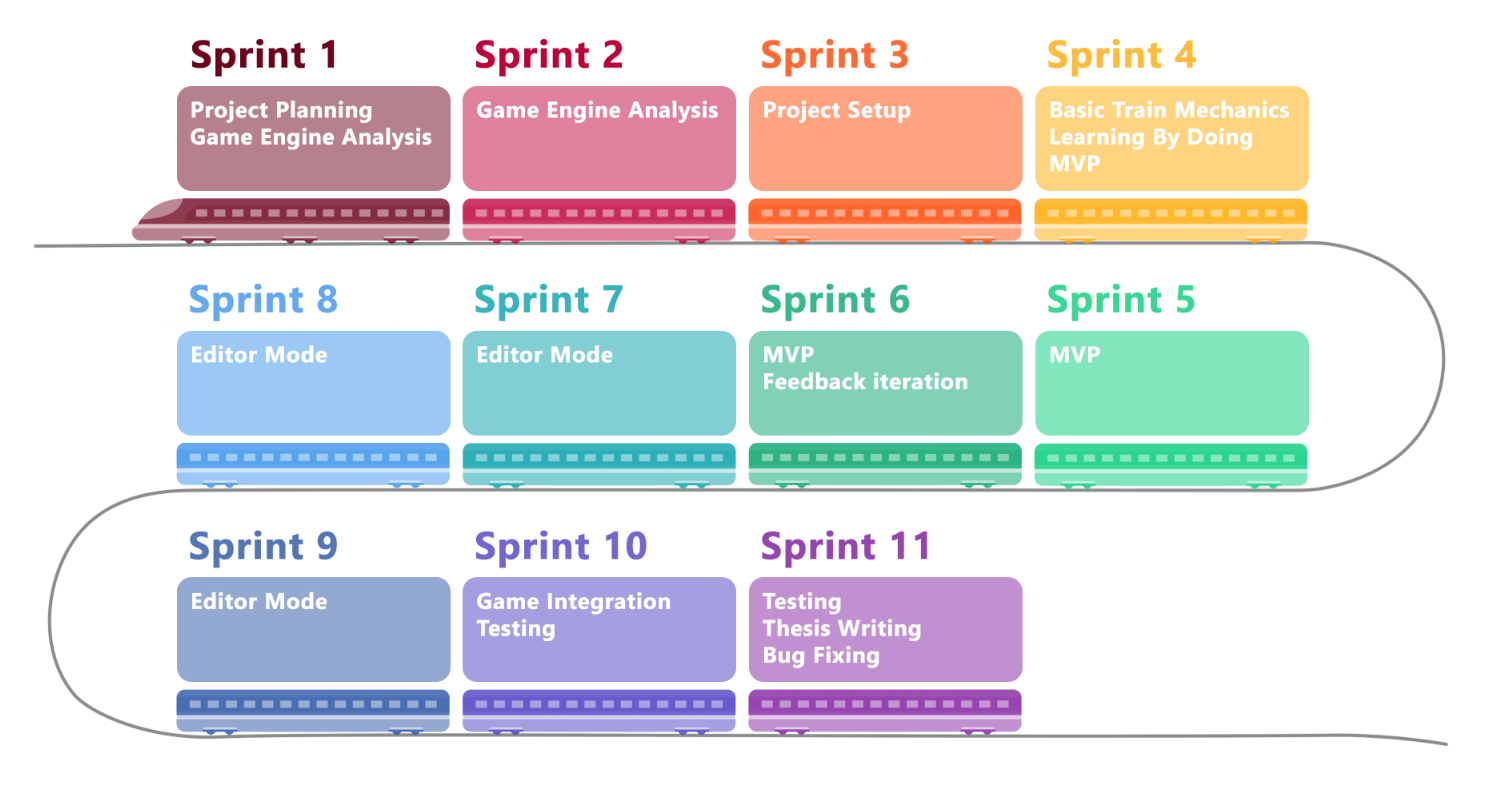
\includegraphics[width=14cm]{figures/ExampleSprintOverview.png}
    %\vspace{-12pt}
    \caption{Overview of all Sprints}
    \label{sprint_overview_img}
\end{figure} 

The scrum meetings are written with three different sections. A section about the Goals we have for the sprint. A section we write when the sprint is completed, which covers the result of the sprint. And a retrospective section where we will discuss and reflect on the result of the sprint with the goals in mind. \\

\textbf{Statuses} \\
The issues in a sprint can be set to one of five different statuses. The statuses are respectively: \textbf{Wishlist} - The issues that is taken out of the project scope and in to a list of functionality that we can decide to include if we have time later in the project. \textbf{To Do} - This are the section for issues that are waiting to be developed. \textbf{In Progress} - The issues that are currently being developed. \textbf{Done} - The issues that has been completed in the sprint.
\\


\begin{large}
\textbf{Sprint 4} \\
\end{large}
\textbf{Date:} 14.02.2022 \\ 
\textbf{Present:} Endre, Henrik, John Ole and Thomas \\
\textbf{Period:} 14.02 - 21.02 \\ 
\\
\begin{table}[H]
    \centering
    \begin{tblr}{
      colspec={|X[0.20, c]|X[0.20, c]|X[0.25, c]|X[0.35, c]|}, hlines,
      column{1} = {gray9},
      column{2} = {blue9},
      column{3} = {yellow9},
      column{4} = {green9},
    }
    \SetCell{bg=gray4}  
    & \textbf{To do} 
    & \textbf{In progress}  
    & \textbf{Done} \\
    Issues 
    & \SetCell[c=1]{l}  Railway integration (7) \newline \newline Curvature warnings (7)
    & \SetCell[c=1]{l} Environment: \newline - Modeling (7) \newline  - Texturing (3)  \newline - Foliage (3) \newline \newline Basic statuses (3)
    & \SetCell[c=1]{l} Input Handling (7) \newline \newline Calculate acceleration (3) \newline \newline Move along Path (7) \newline \newline Signals: \newline \newline Add Models (3) \newline \newline Railway: \newline \newline - Procedural mesh (7) \newline \newline Spline Formation (14) \\
        Estimates & 14 & 16 & 41 
    \end{tblr}
\end{table} 
\bigskip \bigskip

\textbf{Sprint Goal:} \\
\begin{itemize}
    \item Finish the basic train mechanics
    \item Finish the first MVP level environment
    \item Finish the Basic spline railway
\end{itemize}

\textbf{Sprint result:} \\
We set out the sprint with very high expectations because of the delays we have had in previous sprints. All the basic train mechanics and the railway got finished as well as some of the environment and signals. 

\textbf{Retrospective:} \\
One of the group members lost some work days because of sickness. We underestimated the time it takes too model, texture and set up foliage for the environment. Thees tasks should each have been estimated as a 3 and is together with the sickness the reason we did not finish all tasks this sprint. We decided to re-estimate the tasks left from the previous sprint and therefore all of the environment tasks will be set as 3 and the basic statuses will also be set on 3. Basic statuses involves more complex functionality than first expected. 

We had a plan to use the estimations of 1 = 3 hours, 2 = 7 hours and 3 = 14 hours, but we decided to change this. The reason we want to change the estimation is because we feel that it is not accurate enough and we should not restrict our estimation process to only three categories. We therefore decided that further estimations should be done by hours alone and not by a predetermined scale.


\begin{large}
    \textbf{Sprint 5} \\
\end{large}
\textbf{Date:} 21.02.2022 \\ 
\textbf{Present:} Endre, Henrik, John Ole and Thomas \\
\textbf{Period:} 21.02 - 28.02 \\ 
\newline
\begin{table}[H]
    \centering
    \begin{tblr}{
      colspec={|X[0.15, c]|X[0.21, c]|X[0.21, c]|X[0.21, c]|X[0.21, c]|}, hlines,
      column{1} = {gray9},
      column{2} = {purple9},
      column{3} = {blue9},
      column{4} = {blue9},
      column{5} = {green9},
    }
    \SetCell{bg=gray4}  &
    \textbf{Wishlist} &
    \textbf{To do} &
    \textbf{In progress} &
    \textbf{Done} \\
        Issues 
        & \SetCell[c=1]{l} Curvature Warnings (10)
        & \SetCell[c=1]{l} Speed Limit Indicator (10) \newline \newline Signals: \newline  - Railway Integration (4)
        & \SetCell[c=1]{l} Basic Statuses (20) \newline \newline Environment:
        - Modeling (14) \newline - Texturing(12) \newline - Foliage(12) \newline \newline Add Speedometer(8)
        & \SetCell[c=1]{l} Drone Mode (7) \newline \newline Spline Terrain Adaptation (10) \newline \newline Main Menu (7) \newline \newline Popup Message (3) \newline \newline In Game Menu (4) \newline \newline Options Menu (10)\\
        Estimates & 10 & 14 & 66 & 41
    \end{tblr}
\end{table}
\bigskip \bigskip

\textbf{Sprint Goal:} \\
\begin{itemize}
    \item Finish Main Menu in game menu and pop-up messages
    \item Finish basic statuses
    \item Finish The environment creation
\end{itemize}

\textbf{Sprint result:} \\
All the initial UI got finished in blueprints. The environment creation is nearly finished. The basic statuses task was increasing in size because...

\textbf{Retrospective:} \\
The sprint was set to contain 121 work hours, this is all the time we as a group has for a full week since every group member should have 30 hours of work each week.We only finished work hours of about 41 estimated hours. And we estimate that half of the in progress tasks are finished. This puts our completed work to 74 hours. We have underestimated both the time and complexity of several tasks. We have to use this knowledge on further estimations meaning we have to estimate issues with a larger margin of error


\begin{large}
    \textbf{Sprint 6} \\
\end{large}
\textbf{Date:} 28.02.2022 \\ 
\textbf{Present:} Endre, Henrik, John Ole and Thomas \\
\textbf{Period:} 28.02 - 07.03 \\ 
\newline
\begin{table}[H]
    \centering
    \begin{tblr}{
      colspec={|X[0.15, c]|X[0.20, c]|X[0.20, c]|X[0.45, c]|}, hlines,
      column{1} = {gray9},
      column{2} = {purple9},
      column{3} = {blue9},
      column{4} = {green9},
    }
    \SetCell{bg=gray4}  &
    \textbf{Wishlist} &
    \textbf{In progress} &
    \textbf{Done} \\
        Issues 
        & \SetCell[c=1]{l} Speed Limit Indicator (10) \newline \newline
        & \SetCell[c=1]{l} Basic Statuses (5)
        & \SetCell[c=1]{l} Environment Creation: \newline - Moddeling (10) \newline - Texturing (10) \newline - Folaige (10) \newline \newline Add speedometer (4) \newline \newline Requirement specification (20) \newline \newline Status report 1 (10) \newline \newline Signals: \newline - Railway integration (4) \newline \newline Gravel Mesh Under Spline (10) \newline \newline Bug: \newline - Spline hovering above ground (15) \\
        Estimates & 10 & 5 & 93 
    \end{tblr}
\end{table}
\bigskip \bigskip

\textbf{Sprint Goal:} \\
\begin{itemize}
    \item Finish first draft of requirement specification and status report 1.
    \item Finish the MVP scenario
\end{itemize}

\textbf{Sprint result:} \\
The MVP got finished and put together. We had some issues with the environment creation and it's time consumption, but the estimations we made for three environment creation tasks was more accurate than our previous estimations. All the necessary functionality was there to display the MVP to the client except the basic statuses which we only controlled by a timer instead of an controller. The basic statuses only misses a few hours of work and is therefore almost finished.

\textbf{Retrospective:} \\
The sprint goals was achieved, but the basic statuses was only implemented to work with the MVP scenario and not finished to he extent we want in the final product. We want the signals to be controlled by a controller and be able to trigger events. New issues for this will come in the next sprint. We finished 93 work hours in the sprint and we feel that our estimations on the different tasks are beginning to get better and more accurate to how we progress in the sprints. We decided after this retrospective meeting to increase the size of the sprints from one to two weeks for the upcoming sprints. We are now going to work on two milestones simultaneously and feel that a two week sprint will give us time to produce more and that the development will be more efficient. 



\begin{large}
    \textbf{Sprint 7} \\
\end{large}
\textbf{Date:} 07.03.2022 \\ 
\textbf{Present:} Endre, Henrik, John Ole and Thomas \\
\textbf{Period:} 07.03 - 21.03 \\ 
\newline
\begin{table}[H]
    \centering
    \begin{tblr}{
      colspec={|X[0.15, c]|X[0.21, c]|X[0.21, c]|X[0.21, c]|X[0.22, c]|}, hlines,
      column{1} = {gray9},
      column{2} = {purple9},
      column{3} = {blue9},
      column{4} = {blue9},
      column{5} = {green9},
    }
    \SetCell{bg=gray4}  &
    \textbf{Wishlist} &
    \textbf{To do} &
    \textbf{In Progress} &
    \textbf{Done} \\
        Issues 
        & \SetCell[c=1]{l} Editor mode: \newline - Generate flat terrain (14) \newline - Manipulate terrain (20) \newline - Dynamic buttons (10)
        & \SetCell[c=1]{l} Place and edit railway (28) \newline \newline Load scenario from file (14) \newline \newline Save scenario to file (14) Static Buttons on screen (7)
        & \SetCell[c=1]{l} Main Goal: \newline - Signal Controller (21) \newline - Emergency Breaks (7) \newline - Stop Scenario (21) \newline \newline In game content browser (25) \newline \newline Save Object to File (20) \newline \newline Load Object From File (20)
        & \SetCell[c=1]{l} Main Menu (14) \newline \newline Basic Statuses (7) \newline \newline Second iteration Requirement Specification (21)  \newline \newline Place 3D Models (12) \newline \newline Manipulate 3D Models (25)  \\
        Estimates & 44 & 63 & 114 & 79
    \end{tblr}
\end{table}
\bigskip \bigskip

\textbf{Sprint Goal:} \\
\begin{itemize}
    \item Finish first draft of requirement specification and status report 1.
    \item Finish the MVP scenario
\end{itemize}

\textbf{Sprint result:} \\
The MVP got finished and put together. We had some issues with the environment creation and it's time consumption, but the estimations we made for three environment creation tasks was more accurate than our previous estimations. All the necessary functionality was there to display the MVP to the client except the basic statuses which we only controlled by a timer instead of an controller. The basic statuses only misses a few hours of work and is therefore almost finished.

\textbf{Retrospective:} \\
The sprint goals was achieved, but the basic statuses was only implemented to work with the MVP scenario and not finished to he extent we want in the final product. We want the signals to be controlled by a controller and be able to trigger events. New issues for this will come in the next sprint. We finished 93 work hours in the sprint and we feel that our estimations on the different tasks are beginning to get better and more accurate to how we progress in the sprints.


\begin{large}
    \textbf{Sprint 8} \\
\end{large}
\textbf{Date:} 22.03.2022 \\ 
\textbf{Present:} Endre, Henrik, John Ole and Thomas \\
\textbf{Period:} 22.03 - 04.04 \\ 
\newline
\begin{table}[H]
    \centering
    \begin{tblr}{
      colspec={|X[0.15, c]|X[0.21, c]|X[0.21, c]|X[0.21, c]|X[0.22, c]|}, hlines,
      column{1} = {gray9},
      column{2} = {purple9},
      column{3} = {blue9},
      column{4} = {blue9},
      column{5} = {green9},
    }
    \SetCell{bg=gray4}  &
    \textbf{Wishlist} &
    \textbf{To do} &
    \textbf{In Progress} &
    \textbf{Done} \\
        Issues 
        & \SetCell[c=1]{l} Editor mode: \newline - Save Scenario to File (14) \newline - Load Scenario from File (20) 
        & \SetCell[c=1]{l}Static Buttons on Screen (7) \newline \newline Place and Edit railways (28)
        & \SetCell[c=1]{l} Save Object to File (20) \newline \newline Load Object From File (20) \newline \newline Log In: \newline - Add User Types (10) \newline - Restrict functionalities (10)
        & \SetCell[c=1]{l} Main Goal: \newline - Signal Controller (21) \newline - Emergency Breaks (7) \newline - Stop Scenario (21) \newline \newline In game content browser (15)  \newline \newline Third Iteration Requirement Spesification (10)\\
        Estimates & 34 & 35 & 60 & 74
    \end{tblr}
\end{table}
\bigskip \bigskip

\textbf{Sprint Goal:} \\
\begin{itemize}
    \item Finish the editor mode, meaning the content browser and all the tools for saving, placing and the UI.
    \item Finish the third iteration of the requirement specification.
    \item Finish the Main Goal which is a working scenario with a controller for the signals.
\end{itemize}

\textbf{Sprint result:} \\
We finished the third iteration of the requirement document and the main goal. The editor mode is about halfway done. 

\textbf{Retrospective:} \\
The estimations we made was not very accurate to the workload. the content browser for example has been challenging to get working. This is because it introduced many problems that we did not account for when estimating. This issue which we thought initially would take approximately 4 days to complete has now been a work in progress for about two weeks. Because of the troubles we have had we will use the next sprint (which includes the easter) to continue working towards finishing up the editor mode.

\begin{large}
    \textbf{Sprint 9} \\
\end{large}
\textbf{Date:} 04.03.2022 \\ 
\textbf{Present:} Endre, Henrik, John Ole and Thomas \\
\textbf{Period:} 04.04 - 13.04 \\ 
\newline

\begin{table}[H]
    \centering
    \begin{tblr}{
      colspec={|X[0.15, c]|X[0.42, c]|X[0.43, c]|}, hlines,
      column{1} = {gray9},
      column{2} = {blue9},
      column{3} = {green9},
    }
    \SetCell{bg=gray4}  &
    \textbf{In Progress} &
    \textbf{Done} \\
        Issues 
        & Place and Edit railways (28)
        & \SetCell[c=1]{l} Save Object to File (5) \newline \newline Load Object From File (5) \newline \newline Log In: \newline - Add User Types (7) \newline - Restrict functionalities (7) \newline \newline Static buttons on screen (25) \newline \newline Fourth iteration Requirement Specification (10) \newline \newline Bachelor Thesis draft (20) \\
        Estimates & 28 & 79
    \end{tblr}
\end{table}
\bigskip \bigskip

\textbf{Sprint Goal:} \\
\begin{itemize}
    \item Finish the editor mode, meaning the content browser and all the tools for saving, placing and the UI.
    \item Finish the fourth iteration of the requirement specification and deliver a draft of the thesis.
\end{itemize}

\textbf{Sprint result:} \\
We finished both the requirement specification and the requirement specification. The place and edit railway issue was started but there was some issues with the relevancy and meaning of including it in the project. 

\textbf{Retrospective:} \\
On our meeting with the supervisor he brought up that it may be necessary to cut out the railway editing tool. Our discussion on the subject. We figured that because of the problems we have had with it and the fact that the functionality we can produce would not be better than using the original spline tool in the UE4 editor we decided that Thomas will work on the issue for one more day to see find out if the issue is worth resolving or if it's smarter to cut out the functionality and focus on other parts of the project.
Update, the place and edit railways issue will be excluded from the backlog because we want to focus on other parts of the assignment.

%%%%%%%%%%%%%%%%%%%%%%%%%%%%%%%%%%%% SCRUM %%%%%%%%%%%%%%%%%%%%%%%%%%%%%%%%%%%%%%%%%%



\subsection{Deviation from original plan}
\bigskip
\begin{figure}[H]
    \centering
    \vspace{12pt}
    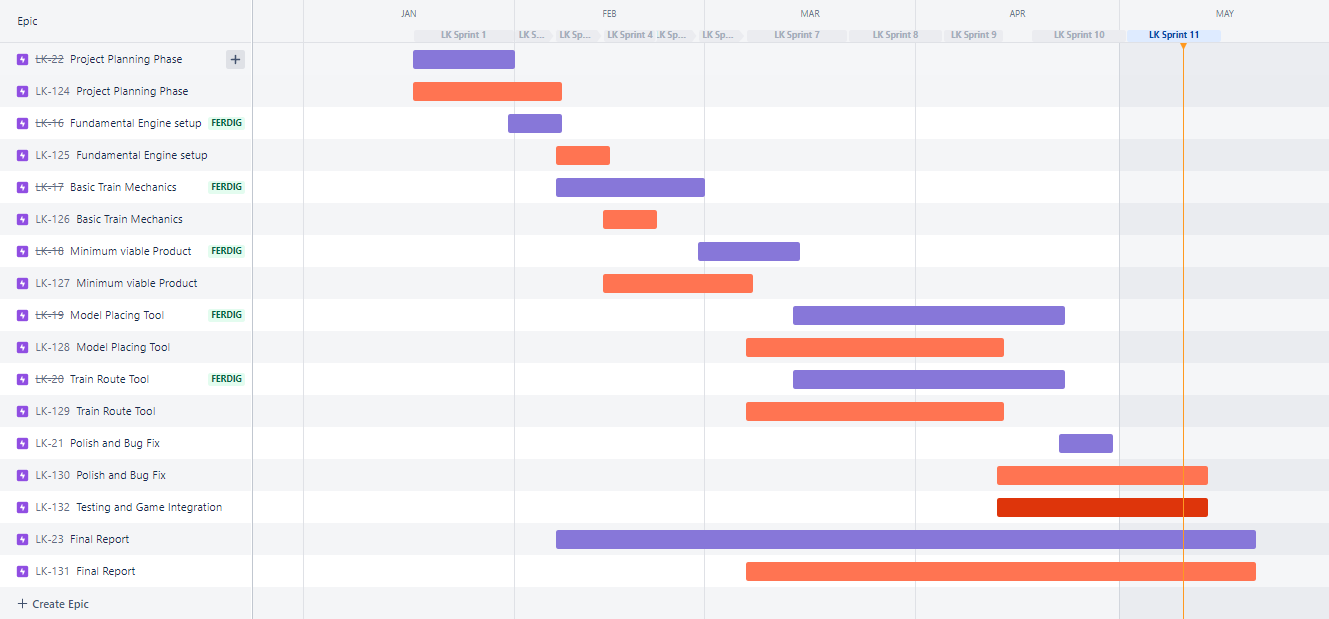
\includegraphics[width=12cm]{figures/Jira comparisoncroped.png}
    \caption{Comparison of }
    \label{Epic_comparison_img}
\end{figure} 
\bigskip \bigskip




- stopped doing daily meetings, felt it was not needed - most meetings were spent repeating already known info 

- after the main goal mvp was done we switched from 1 week to 2 week sprints, as we felt the tasks ahead required more time to develop and progress. using 2 week sprints allows the group to take a day off after a sprint to work on other stuff unrelated to the issues in the sprint if they want. When having 1 week sprints the time spent developing vs time spent planning is (not enough we feel). 


\section{Deployment}

\subsection{Packaging and release}
%

Using the packaging system in Unreal. Project is exported and saved with exe and .pak files containing content. The whole folder can then be zipped and uploaded to a server. The zip can be downloaded and unzipped in a folder, and the game should work without further installation. When the game is updated it would need to be packaged again and re-downloaded with the current setup. This method is also what is currently in use at Lokførerskolen.

One option to improve the update process is to create an auto-updater, and automatically patch the game with new updates. Doing this would most likely require more work than it is worth if the game is not updated often. In Unreal it is possible to use clustering in the pak files, which allows for easier streaming and patching of game data. 
\section{Implementation} % Slå sammen implementasjon og design? enklere å snakke om et "tema" istedenfor å dele det opp

% design skal være hvordan vi designer systemet vårt, kinda litt som high-level usecase hvor vi beskriver hvordan ting skal virke for brukeren, mens design viser hvordan det ca skal sitte sammen logikk wise. Implementation skal være spesifikt hvordan vi har gjort det med kode, så må nesten være separate

This section will look closer into the ideas, code and structure behind various parts of the application. all shown code is written by the project group members. One important aspect of Unreal Engine to remember is that the order of axes might be different than other industry standards, as Unreal Engine uses a Left Handed, Z Up coordinate system. (source) In this three-dimensional space, the \textbf{X}-axis points forwards, the \textbf{Y}-axis points to the right, and the \textbf{Z}-axis points upwards. 

\subsection{Spline Tool}

One of the first goals specified by the client was to move the train along a straight path. Seeing as a later goal was to also implement curvature, we decided that it would be beneficial to begin work on curved train movement right away, as this would likely save us some time. In the existing simulator, the railway is procedurally generated from a list of points forming a \textit{spline}. A spline can be defined as a mathematical function to interpolate and form a smooth curve between multiple points. Each point is made up of a location vector and a tangent vector for specifying the curvature of the spline at the given position. We also looked into \textit{Bézier curves}, a similar alternative to splines, but Unreal Engine's built-in spline component made it an obvious choice. \newline

\begin{figure}[h]
    \centerline{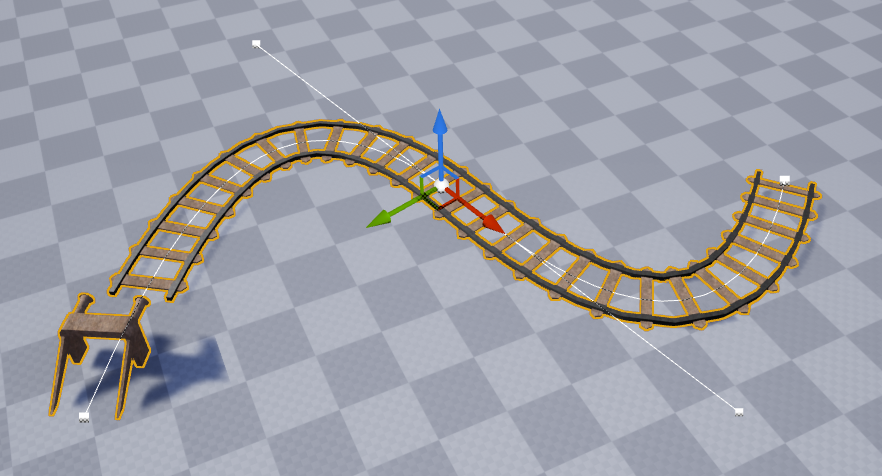
\includegraphics[width=0.9\textwidth]{figures/Spline1.png}}
    \caption[size=small]{A selected spline deforming a railway mesh along itself. The white squares indicate the spline points, and the white lines indicate the tangent of the selected spline point.}
\end{figure} 


We created \textit{ASplineActor}, a class for handling all functionality related to the railway. This class contains a \textit{USplineComponent}, a powerful component with functions for placing and deforming a mesh along a spline. In this context, a mesh can be described as a 3D-model. The way this initially works is by looping over all points in the spline, placing a sub-mesh that is stretched between points $P_n$ and $P_{n+1}$, and bending the meshes by the curvature of the tangents between $T_n$ and $T_{n+1}$. The spline points were defined by the user in the editor, and could be placed freely. The results looked promising, but a major flaw of this method occurs when any distances between each set of spline points aren't uniform. The meshes would stretch differently along the spline, making the railway look rather odd. A good analogy is imagining a skyscraper with a single, horizontally stretched window instead of separate windows on each floor. The solution to this was to split the spline into segments of equal length to that of the mesh/model itself, and add a new sub-mesh at each segment. Essentially cutting up the railway into pieces and replacing the existing spline points. The mesh used in figure \textbf{X} is a small slice of a railway created with primitive shapes in Asset Forge. \\

% CODE

% SKAL FJERNE MASSE AV KODEN DONT WORRY

\begin{code}

// Get the size vector of the mesh
const FVector MeshSize = Mesh->GetBoundingBox().GetSize();
	
// Get the length of the bounding box of the mesh along the forward axis
const float MeshLength = MeshSize.X;

...

const float SplineLength = SplineComponent->GetSplineLength();

// Set number of spline points to number of meshes fitting inside spline length
const int SplinePoints = FMath::CeilToInt(SplineLength / MeshLength);

for (int PointCount = 0; PointCount < SplinePoints; PointCount++)
{
	// Generate a spline mesh component for each point in the spline
	USplineMeshComponent* SplineMesh = 
	NewObject<USplineMeshComponent>(
	    this, USplineMeshComponent::StaticClass()
	);

	...
	
	// Get the location and tangents for the mesh at the 
	// current distance along the spline
	
	const float StartDistance = MeshLength * PointCount;
	
	FVector StartPoint = GetLocationAtDistanceAlongSpline(
	    StartDistance, ESplineCoordinateSpace::Local
    );
	    
	FVector StartTangent = GetDirectionAtDistanceAlongSpline(
	    StartDistance, ESplineCoordinateSpace::World
    );
    
	// Get the location and tangents for the end of the 
	// mesh at the current distance along the spline

	const float EndDistance = MeshLength * (PointCount + 1);
	
	FVector EndPoint = GetLocationAtDistanceAlongSpline(
	    EndDistance, ESplineCoordinateSpace::Local
	);
	
	FVector EndTangent = GetDirectionAtDistanceAlongSpline(
	    EndDistance, ESplineCoordinateSpace::World
	);
	
	...
	
	// Set the mesh location and curvature in spline
	SplineMesh->SetStartAndEnd(
	    StartPoint, 
	    StartTangent, 
	    EndPoint, 
	    EndTangent
    );
}
\end{code}
%\caption[size=small]{KODE! :D}

Opting for a custom spline class instead of Unreal Engine's solution let us change the spline into a railway, adding specific elements such as \textit{buffer stops}, the metal bars at the end of a railway to stop trains. We added an optional parameter to the ASplineActor class, where the user can input a separate mesh to be displayed as the first and/or the last sub-mesh of the spline. However, if this field is left empty, the sub-mesh will default to the given railway mesh. We also implemented a boolean flag which sets off if the spline extends a desired angle or curvature limit, to ensure the train looking natural when traversing the railway. \newline

\begin{figure}[h]
    \centerline{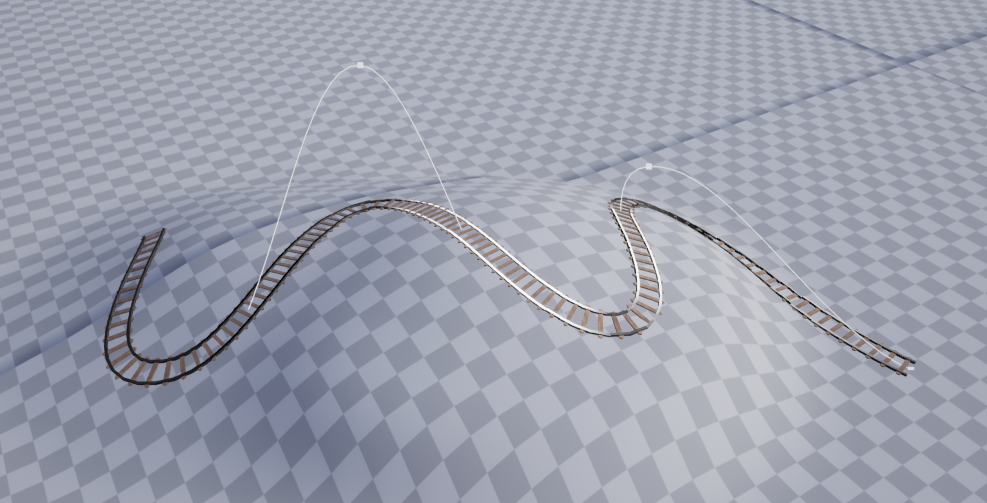
\includegraphics[width=0.9\textwidth]{figures/Spline2.png}}
    \caption[size=small]{A railway conforming to the terrain height}
\end{figure} 

One of the challenges with the tool occurred when manually placing the spline points. The railway curved naturally in the horizontal plane, but if the terrain had any difference in height, the railway would simply disappear under ground or hover above ground. To solve this, we perform a line cast in each spline point's X and Y coordinates, from the top to the bottom of the level. This is a way to see if we hit any terrain along the line cast. If there is a hit, the Z-coordinate of the relevant spline point is simply set to the height value of the terrain hit. This gets more computationally expensive the longer a spline is, but is only run once when a spline undergoes change, so any noticeable effects are minuscule. 
% kjør oppdatering av spline i en annen thread? da slipper editoren å lagge så mye når man endrer på ting. fant en plugin som bruker spline greier i en annen thread, men koster penger. Skal gå ann å lage en ny thread, gjøre computations der og sende det tilbake i game thread. - EH

\subsection{Signal controller}

The Central Signal Controller is responsible for signal and status communication between the signals and trains. The controller receives signal and status updates from TriggerBoxes, which are placed along the railway and are used to send signal or status updates depending on configured conditions. 

When the level is loaded and the game begins, the Central Signal Controller searches for all actors inheriting from the Basic Signal class. Valid actors are then sorted into lists based on which type they are, such as Main Signal or Forward Signal. These different lists are then used later to send signal updates. 

% vis kode som søker etter og lagrer actors fra central signal controller
\begin{code} 
void ACentralSignalController::FindAllSignals()
{
	// Finds all actors of signal classes
	UGameplayStatics::GetAllActorsOfClass(GetWorld(), DwarfSignalBP, DwarfSignalActors);
	UGameplayStatics::GetAllActorsOfClass(GetWorld(), MainSignalBP, MainSignalActors);
	UGameplayStatics::GetAllActorsOfClass(GetWorld(), ForwardSignalBP, ForwardSignalActors);

	int32 i = 1;

	// Loops through all actors
	for (AActor* DwarfSignalActor : DwarfSignalActors)
	{
		ABasicSignal* DwarfSignal = Cast<ABasicSignal>(DwarfSignalActor);
		if (DwarfSignal)
		{
			FString TagName = FString::Printf(TEXT("Dwarf_%i"), i++);
			
			DwarfSignal->Tags.Add(FName(TagName));

			AllSignalActors.Add(DwarfSignalActor);
		}
	}
	...
}
\end{code}

When the controller receives a signal update, an ID, new signal state and signal type must be specified. The controller then searches through the specified signal list to match the IDs, and when this happens the new signal state is sent. The controller continues searching the list, if more than one signal shares the same ID. Given that the length of the list of signals is quite short, the time spent searching the list even when the first match is found is insignificant. % measure this? or at least prove the time spent will have a small to none effect on fps

% vis kode som finner riktig signal og sender signalet
\begin{code}
void ACentralSignalController::SendUpdatedSignal(FName SignalID, ESignalType SignalType, ESignalStatus Status)
{
	TArray<AActor*> Actors;

	// Selects relevant actors to search based on signal type
	switch (SignalType)
	{
	case ESignalType::Main:
		Actors = MainSignalActors;
		break;
	case ESignalType::Forward:
		Actors = ForwardSignalActors;
		break;
	case ESignalType::Dwarf:
		Actors = DwarfSignalActors;
		break;
	default:
		checkNoEntry();
		break;
	}

	// Loops through all signals
	for (AActor* SignalActor : Actors)
	{
		ABasicSignal* Signal = Cast<ABasicSignal>(SignalActor);
		if (Signal && (Signal->ID == SignalID))
		{
			// If the signal matches the incoming id, update the status
			Signal->UpdateSignalStatus(Status);
		}
	}
}
\end{code}

As the Central Signal Controller is an actor, it needs to be placed in every level which is going to use signals. One alternative would be to create a subsystem with the same functionality. This would allow the controller to work in any level without needing to place an actor, as well as having a more predictable and stable lifecycle. 

\subsection{Signals}

The class ABasicSignal is used for the three different types of signals. The three signal types share the same functionality, with the only difference being the models used and number of lights on each model, as well as which colors are used and how the signal reacts to signal status updates. 

% vise bilde av blueprint kode som bestemmer signal status greier

different models have different numbers and locations, so automatic light creation and placement is used

dynamic signal creation at runtime, uses sockets to place signal lights, emissive lights used

% vise kode som lager lysene på signalene
\begin{code}
void ABasicSignal::SetupLight()
{
	RemoveLights();

	// Create all lights in a loop
	for (int32 i = 0; i < NumLights; i++)
	{
		FString SocketName = FString::Printf(TEXT("Socket_%i"), i + 1);
		FString LightMeshName = FString::Printf(TEXT("LightMesh_%i"), i + 1);

		UStaticMeshComponent* LightMesh = NewObject<UStaticMeshComponent>(this, FName(LightMeshName));

		// Creates a new light struct
		FSignalLight NewLight(LightMesh);

		NewLight.LightMesh->SetStaticMesh(BaseLightMesh);

		NewLight.LightMesh->SetupAttachment(VisualComponent, FName(SocketName));

		// Creates the instanced dynamic light material
		NewLight.DynMaterial = UMaterialInstanceDynamic::Create(BaseLightMaterial, this);

		NewLight.DynMaterial->SetScalarParameterValue("Emissive_Strength", MaxLightLevel);
		NewLight.DynMaterial->SetVectorParameterValue("Emissive_Color", FLinearColor(1.0f, 1.0f, 1.0f));

		NewLight.LightMesh->SetMaterial(0, NewLight.DynMaterial);

		NewLight.LightMesh->RegisterComponent();


		Lights.Add(NewLight);
	}
}
\end{code}

registers new component, otherwise the object is garbage collected

creates a new dynamic material instance to give each light its own color and properties

\subsection{Editor Mode}
The goal of the editor mode was to give the client a simple tool build worlds and train scenarios. Our task was to implement the ability to place, move and rotate objects such as trains and buildings, and a way to lay a railway across the terrain. We decided to design this tool based on the tools available in Unreal Engine's own editor, as these would accomplish similar tasks. For moving objects around, we created a \textit{gizmo} consisting of one arrow for each axis, and a square for the plane along the X- and Y-axes. Once an object is selected, this gizmo appears at its position, utilizing custom depth rendering, which enables the gizmo to always be visible even when it is covered by another mesh. 

\begin{figure}[h]
\centering
\begin{minipage}{.5\textwidth}
  \centering
  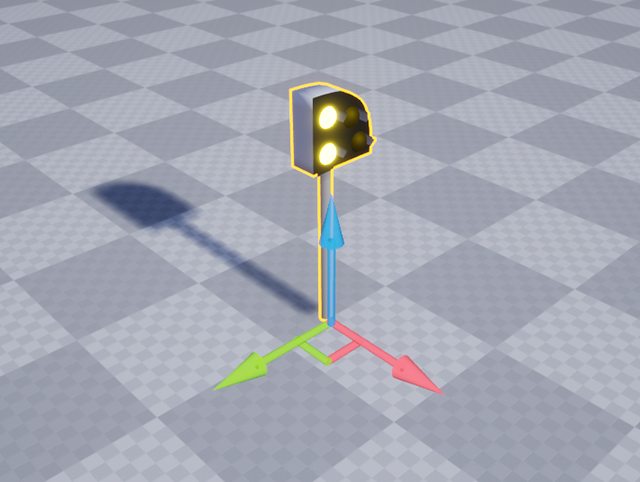
\includegraphics[width=0.95\linewidth]{figures/Gizmo1.png}
  \captionof{figure}{The translation gizmo on a selected signal}
  \label{fig:test1}
\end{minipage}%
\begin{minipage}{.5\textwidth}
  \centering
  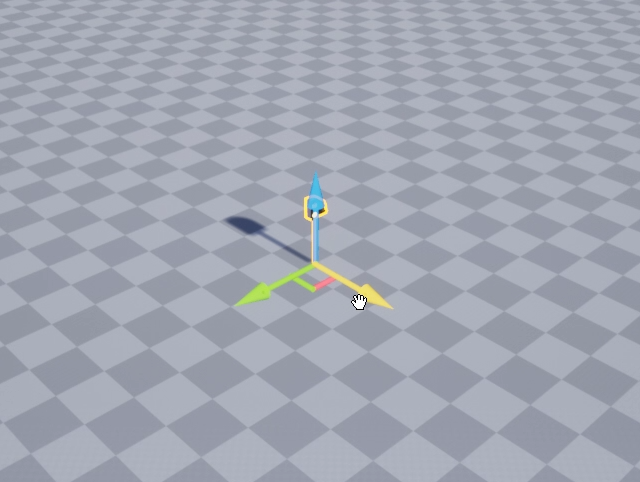
\includegraphics[width=0.95\linewidth]{figures/Gizmo2.png}
  \captionof{figure}{The translation gizmo far away, hovering the X-axis arrow}
  \label{fig:test2}
\end{minipage}
\end{figure}

By hovering the mouse over one of the gizmo's arrows and dragging, the user can move the object in the relevant axis. This is done by casting a line from the camera, in the direction of the cursor's position on the screen, and processing the results on hit. This is done in a separate collision layer for gizmos, such that the line is not obscured by any object. The tool includes two modes, translation and rotation. When switching mode to rotation, the arrow meshes are replaced by a cogwheel in the X-Y axis plane, which rotates the object around the Z axis when dragged. These gizmos are made to be a part of the user interface, and get scaled based on their distance from the camera to keep their size uniform. 

When grabbing a gizmo arrow to move an object, the position of the cursor is saved as a variable in the first frame of holding down the mouse button. This position is used to get the offset between the gizmos center position (also the object anchor position), and the cursor. While dragging the gizmo arrow, the objects position is set to the location of the cursor minus the offset, resulting in the object moving in parallel with the cursor. This behaviour works fine in theory, but during testing, we found a lack of user friendliness due to the cursor having to overlap the gizmo during dragging. To combat this, we added secondary meshes to each arrow that would inflate the area of interaction. These meshes were given an invisible material, so the user could not see them, but were able to interact with them.

\begin{figure}[h]
\centering
\begin{minipage}{.5\textwidth}
  \centering
  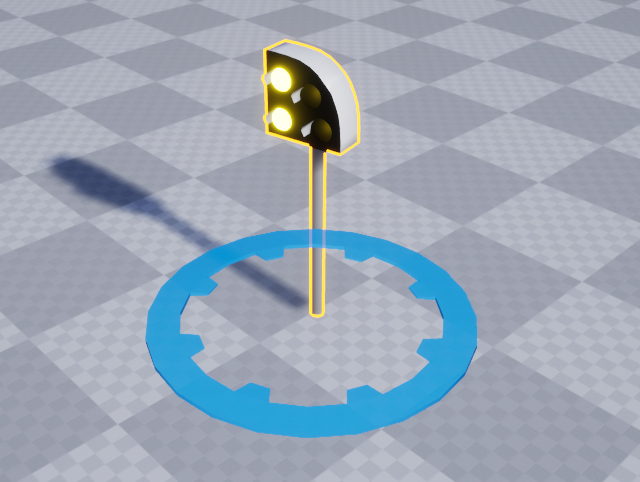
\includegraphics[width=0.95\linewidth]{figures/Gizmo3.png}
  \captionof{figure}{The rotation gizmo in the X-Y plane}
  \label{fig:test1}
\end{minipage}%
\begin{minipage}{.5\textwidth}
  \centering
  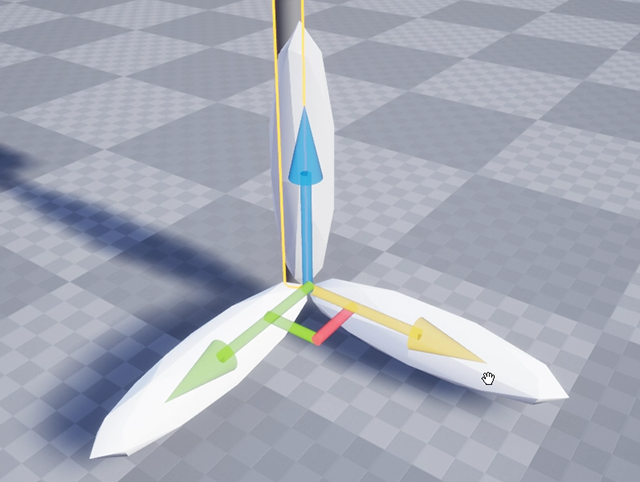
\includegraphics[width=0.95\linewidth]{figures/Gizmo4.png}
  \captionof{figure}{Additional meshes around the arrows}
  \label{fig:test2}
\end{minipage}
\end{figure}

During user testing with the client, it was made clear that this interaction was still hard, as the cursor would, more often that not, exit the area of these meshes. This was towards the very end of the development, and there was not enough time to iterate on this implementation, as it would quickly grow complicated. But due to the curious nature of programmer brains, we were attracted towards finding a solution to this problem. Even if we did not have the time to finish the implementation of these ideas, we came up with several possible solution that could fix or recreate this system entirely.

The first idea was to 
\section{Testing}

\subsection{Hardware testing}
% Testing on the hardware the computers at lokførerskolen.

\subsection{Testing methology}
% The continuous testing methodology the group has done and the outcome of this...

\subsection{User Testing}

In collaboration with the client, we set up user tests towards the end of development. We visited The Norwegian Train Driver Academy and borrowed three students who have previously used their current simulation software. The goal of user testing was to further iterate on the software based on given feedback, but we didn't have a lot of time as the testing was done two weeks prior to the deadline. The tests were done by prompting the user with a set of tasks. These were simple tasks, designed to test the user interface, software structure and overall user experience.  The observer measured the time spent, while writing down notes from the user’s performance. The user was also prompted with questions about the experience. \newline

\begin{table}[H]
    \begin{tblr}{colspec={|X[.2, l]|X[.8, l]|}, hlines}
        \textbf{Case 1:} & Start the scenario named "Testing" \\
        \textbf{Preconditions:} & The software is launched \\
        \textbf{Expected execution:} & The subject navigates to the correct tab, and clicks "Testing" \\
        \textbf{Actual execution:} & 
        The first two subjects started by navigating through the main menu tabs to search for "Testing", and clicked it once they saw it. The third subject clicked the correct tab as their first action, but the button did not respond, making the subject believe the scenario was not placed under this tab. This resulted in the subject launching the wrong scenario, making them exit the application to try again. \\
        
        \textbf{Results:} & The subjects complimented the look and feel of the interface. In a later discussion, they all agreed when one of the subjects said the interface was more user friendly than the existing simulator. \\
    \end{tblr}
    \caption{User Test Case 1: Start the scenario named "Testing"}
\end{table}
\bigskip \bigskip \bigskip
\begin{table}[H]
    \begin{tblr}{colspec={|X[.2, l]|X[.8, l]|}, hlines}
        \textbf{Case 2:} & Drive the train \\
        \textbf{Preconditions:} & The subject is familiar with the controls from the existing simulator \\
        \textbf{Expected execution:} & The subject accelerates the train, riding through the whole map \\
        \textbf{Actual execution:} & The subjects, being used to the old simulator, quickly resorted to the controls they were used to, and continued to operate the train.\\
        
        \textbf{Results:} & This case was less structured and more focused on the general feedback from the subjects. We gave them freedom to explore the simulator while asking for their impressions.  \\
    \end{tblr}
    \caption{User Test Case 2: Drive the train}
\end{table}

\begin{table}[H]
    \begin{tblr}{colspec={|X[.2, l]|X[.8, l]|}, hlines}
        \textbf{Case 3:} & Exit the game \\
        \textbf{Preconditions:} & The subject has started a scenario \\
        \textbf{Expected execution:} & The subject presses the "escape"-button, then navigates to the main menu before exiting the game \\
        \textbf{Actual execution:} & All subjects started by pressing the escape key, then clicking "main menu", and "exit". \\
        
        \textbf{Results:} & This went smoothly, as if all subjects had done it before. We received compliments for the simplicity of the menu navigation, and praise for designing it in such a way that there is no need to exit the application when starting another scenario. \\
    \end{tblr}
    \caption{User Test Case 3: Exit the game}
\end{table}

% How to perform the tests.

% Case: Starte TestLevel. kjøre gjennom levelet og fortelle om brukeropplevelsen.

%Forklaring:
%Du har en DMI, viser kun fart og signaler vises kun som fysiske signaler i terrenget.

% Case: Obsewrvasjon: Gi oppgaver og se tidsbruk, forståelse og brukeropplevelse.

% Case 1: Start "Test Level Scenarioet"
%Tidsbruk:
% Beskrivelse: Beskrive hvorfor brukeren ikke klarte oppgaven/brukte lang tid.


% Få toget opp i 80 kmt ved bruk av spakene. 
% Beskrivelse:

% Følge med, Halv fart

% Følge med, Stoppe før stopp signal.

% Naviger tilbake til hovedmenyen

\subsection{System Testing}
System test 02.05.2022 \\
To ensure the quality and resilience of our system some basic tests were performed on the system functionality.  \\

The first test was performed on the entire simulator system which includes all functionality exept the editor mode. When changing the screen resolution and window mode, the application did not perform any actions suggesting that our implementation was wrong. After reviewing our code and searching for the issue online we found the origin of the problem. We did not actually apply the settings we want to change.

\begin{code}
	GEngine->GameUserSettings->ApplyResolutionSettings(false);
\end{code}

The fix to the problem was to call the text block above after changing the resolution settings.

When entering the pause menu from the simulator we found that pressing the p-button did not remove the pause menu which it should. This is not a bug but it just needed to be implemented. \\

The switch to drone mode did not work and after rewieving the code it was found that the key binding in the code did notmatch the specified key binding in the engine. We had to change the name of the key binding in train.cpp to get it to work. \\

The drone camera did not spawn in the right place. Our implementation should spawn the drone camera over the train looking in its forward direction but it seemed to be spawning where it was placed out. This was woking in the MVP so after a review of the code we found out that the reference handling of the train from the drone had changed since the MVP. The solution was to add a function which loops over all train actors in a scene and uses the first train it finds to place the drone. The previous solution had the train as a UPROPERTY, but this implementation would not work if the train as deleted and added again.


System test 02.05.2022 \\
e performed some tests on the editor mode ...





\chapter{End Chapters}
\section{Discussion}
%Sum up tall the goals and to what degree they got achieved. Thees includes learning goals (dev and process), effect goals, resultgoals...

%A section about alternatives, options and choices we made. 

%Maybe a section summing up our experience with unreal as the choice of engine, are the expectations met, why, why not. A critical view on the game engine analysis.
\subsection{Version Control System}
Version control or source control, is the practice of tracking and managing changes to software code often within a development team\cite{what_is_version_control}.

Before we started developing we had to chose what version control system we would use. On one side we have Perforce, often a standard choice for larger studios and is favored within game development due to its handling of large binary files. On the other side we have Git a standard choice for developers all around due to its many features for teams and how it supports multiple branches which helps with cooperation within a team. The biggest structural difference is that Perforce uses a centralized model unlike Git which uses a distributed decentralized model. Deploying a Perforce server is also necessary before you can use it, unlike Git which is ready to be used from a cloud service such as Github or Azure DevOps. 
Throughout our bachelor program we have used Git as a version control system and collaborative tool to help us keep the code base consistent and maintained, and is one of the reasons for using it in this project as well. Git can also be hosted on the cloud through for example Github, which we also used in this project. Although Perforce would probably be a better choice for bigger projects and teams since it can handle bigger files more efficiently\cite{different_version_control_used_in_gamedev}.

The biggest issue we faced with git was its single file size limit of 100MB, since Unreal Engine projects contain bigger files such as 3D models, textures and maps. We had a few instances were a map file containing the level scene were bigger than git`s allowed file size limit. As a fix we used the level layer tool in Unreal Engine to split the level file into multiple smaller map files. This temporary fixed the issue and we were no longer hitting the max file size limit of git, although this also made it possible for us to edit and work on the same level without having to overwrite each others changes, since we could just work on different level layers. This is due to the maps being binary files which git cant merge. You either have to pick the current one or the incoming file when merging, unlike cpp files which can be edited by multiple people and can be properly merged together after. 

We also tried using git LFS at the beginning, although GitHub only provides a LFS storage capacity and bandwidth at 1GB which we quickly used up in one single commit. 

Git has many cloud hosting services were you can create repositories in the cloud, such as Github, Gitlab, Bitbucket or Azure DevOps.
Review of the bachelor, what are the effect this bachelor has in the world. How valid and important are the work we have done. If yes why, if no why not.

\textbf{Ask Tom}
\section{Transferability and usability of the Thesis}

A section on how the product hold up to standards, if it should and can be used further, to what degree.

\section{Group Work Evaluation}
How did we approach the thesis, progress in the beginning and general.

The organizational aspect, how did we work and when. What did we log, how did we log where can the readers find this documentation

The separation of duties. How was work assigned, and how was the general work load balancing within the group. 

How was it to work in the group,m good and bad experiences.

\section{Conclusion}
Summing up the bachelor work as a whole. Remember to have that red line and not bring in any new concepts in this section. 




\chapter*{\bibname}
\printbibliography[heading=none]

\appendix

\label{Prosjektavtale}
\includepdf[pages=-]{appendices/NTNUProsjektavtale.pdf}

\label{CodeConvention}
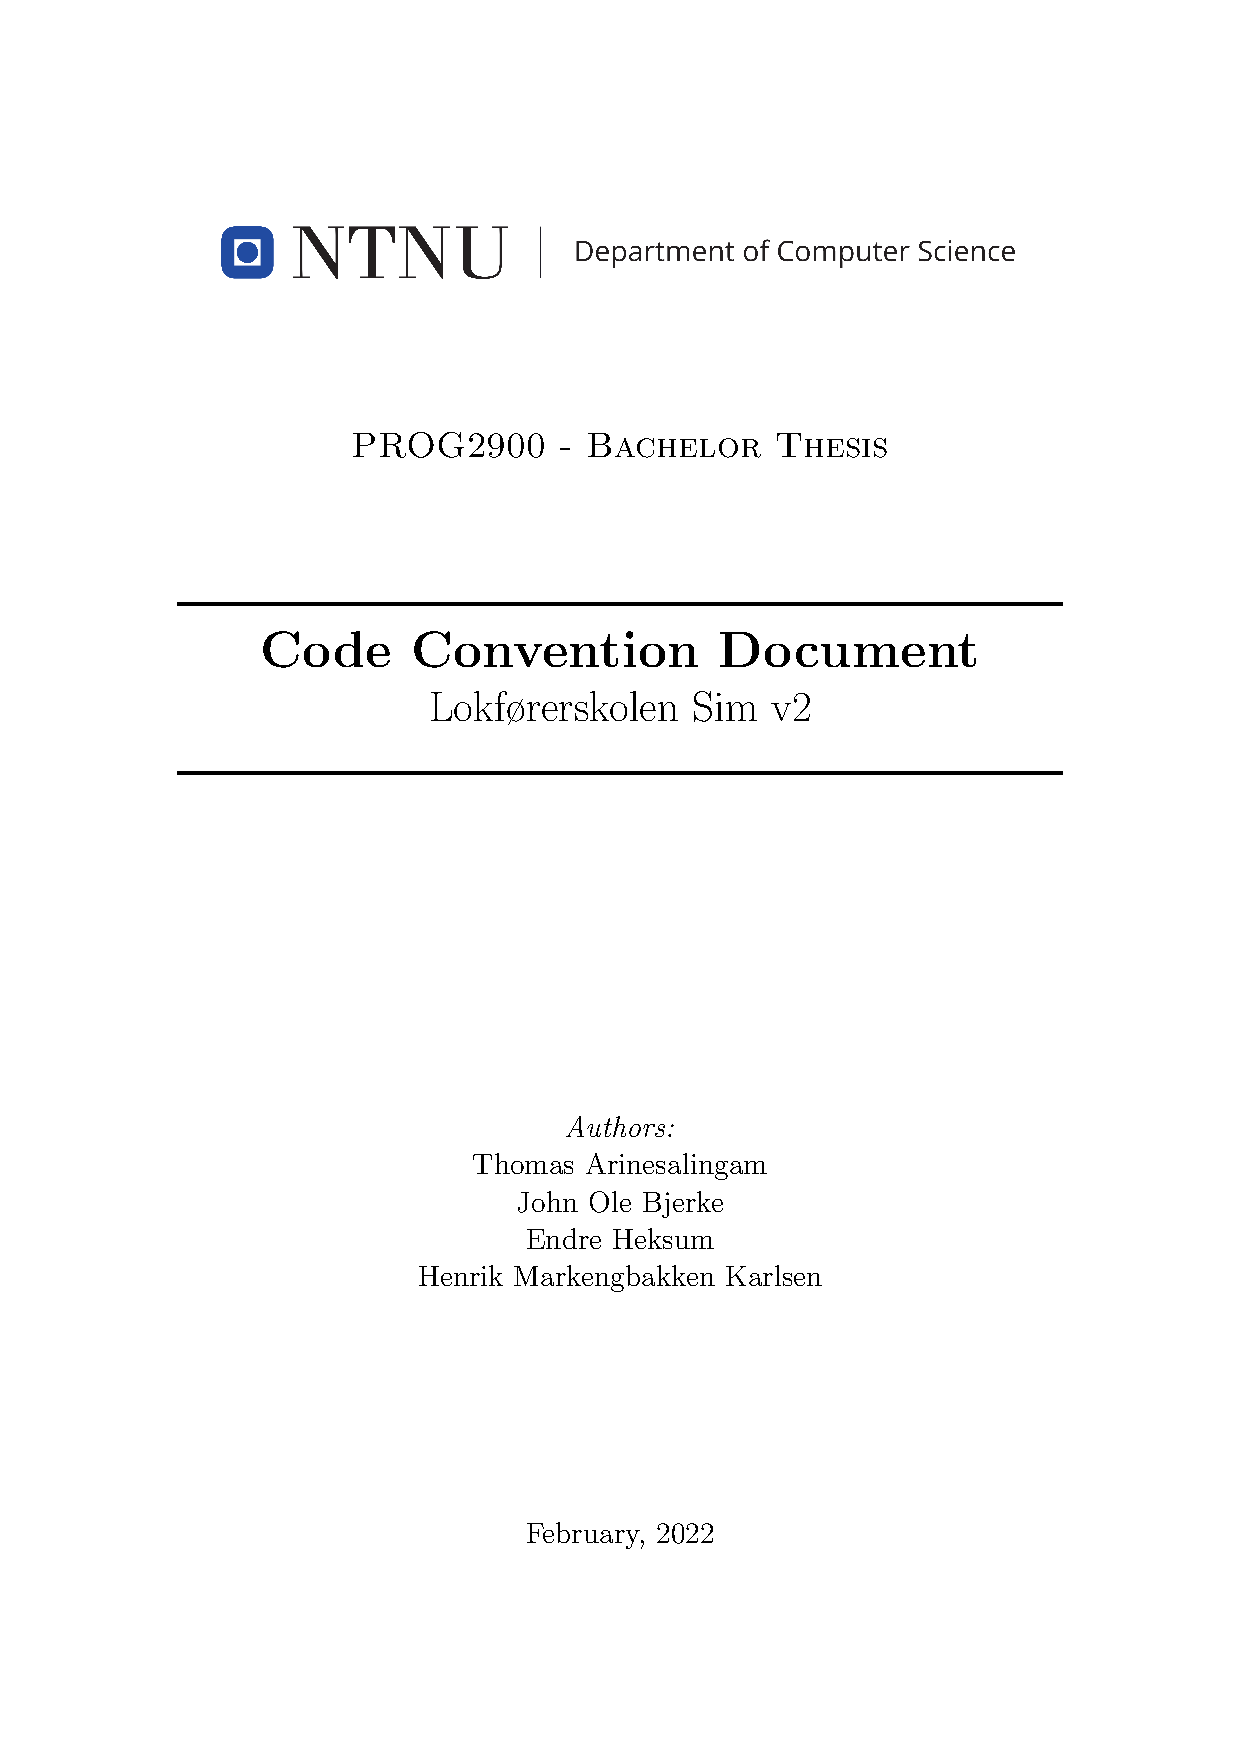
\includepdf[pages=-]{appendices/Code_Convention_Document.pdf}

\end{document}
